\documentclass[12pt]{article}

%preamble%%%%%%%%%%%%%%%%%%%%%%%%%%%%%%%%%%%%%%%
%\usepackage{ctex}
\usepackage{geometry}
\geometry{left=1in,right=0.75in,top=1in,bottom=1in}
\usepackage{pgfplots}
\usepackage{float}
\usepackage{url}
\usepackage{makeidx}
\makeindex
\usepackage{subcaption}
\bibliographystyle{plain}
\usepackage{algorithm}
\usepackage{algpseudocode}
\usepackage{newtxtext}
\usepackage{amsmath,amssymb,amsthm}
\usepackage{newtxmath} % must come after amsXXX
\usepackage{xcolor}
\usepackage{fancyhdr}
\usepackage{appendix}
\usepackage{booktabs}

\lhead{Team \Team}
\rhead{}
\cfoot{}

\newtheorem{theorem}{Theorem}
\newtheorem{corollary}[theorem]{Corollary}
\newtheorem{lemma}[theorem]{Lemma}
\newtheorem{definition}{Definition}[section]

\newcommand{\Problem}{ABCDEF}
\newcommand{\Team}{2400609}

\renewcommand\appendixtocname{Appendix}
%%%%%%%%%%%%%%%%%%%%%%%%%%%%%%%%%%%%%%%%%%%

\begin{document}

\graphicspath{{.}}  % Place your graphic files in the same directory as your main document
\DeclareGraphicsExtensions{.pdf, .jpg, .tif, .png}

%Summary%%%%%%%%%%%%%%%%%%%%%%%%%%%%%
\thispagestyle{empty}
\vspace*{-16ex}
\centerline{\begin{tabular}{*3{c}}
	\parbox[t]{0.3\linewidth}{\begin{center}\textbf{Problem Chosen}\\ \Large \textcolor{red}{\Problem}\end{center}}
	& \parbox[t]{0.3\linewidth}{\begin{center}\textbf{2024\\ MCM/ICM\\ Summary Sheet}\end{center}}
	& \parbox[t]{0.3\linewidth}{\begin{center}\textbf{Team Control Number}\\ \Large \textcolor{red}{\Team}\end{center}}	\\
	\hline
\end{tabular}}

\begin{center}
	\Large \textbf{Shortest Path Algorithms:~Taxonomy and Advance in Research}
\end{center}

As for problem 1,  in order to accurately capture the effective information in the data 
set, we take a series of data processing methods... After that, we select potential influencing
factors and establish Analytic Hierarchy Process (AHP) model to make a preliminary analysis of the influencing
factors and calculate specific parameters for each factor. We find that the biggest factor is 
score difference. Apart from that ,whether scored in the last point, running distance, unforced error and fast win
will also positively or negatively influence the momentum to a comparatively large extent. The above conclusion is verified
in our later models.\\

In problem 2, we believe that momentum will affect the future scores of the match. So to answer the coach's question, 
we first perform autocorrelation test on momentum, and we find that it has strong first-oredr autocorrelation. Then we quantify 
the future scores and then determine the correlation of momentum the scores in the future, they are highly correlated.\\

Problem 3 is devided into 3 parts. To predict the swings in the match , we establish model based on Gated Recurrent Unit(GRU) algorithm.
We process data in problem 1 and add more features. We define the swings and use previous information to predict future.
Then compared to the result in problem 1, our accuracy is ....\\

To identify the most related factors, we use a novel argorithm called Permutation Feature Importance argorithm, 
it can determine the importance of features by calculating their prediction error after permutation. We find that ....\\

As for the ideas for specific atheletes, we use previous model on their matches to identify their feature importance.
We find that different atheletes have different features in their match.\\

Problem 4\\

Key words: AHP, correlation analysis, GRU, Permutation Feature Importance

Indroduction\\
Tennis more than any other sport, is a game of momentum. 
The absence of a clock to do the dirty work of finishing off an opponent, 
and a scoring system basedon units used, makes the flow of the match much more important than any 
lead that has been established.--Chuck Kriese\\

problem3

Using the above argorithm, we sort FI and normalize them, then we plot the figure:

\begin{figure}[H]
    \centering
    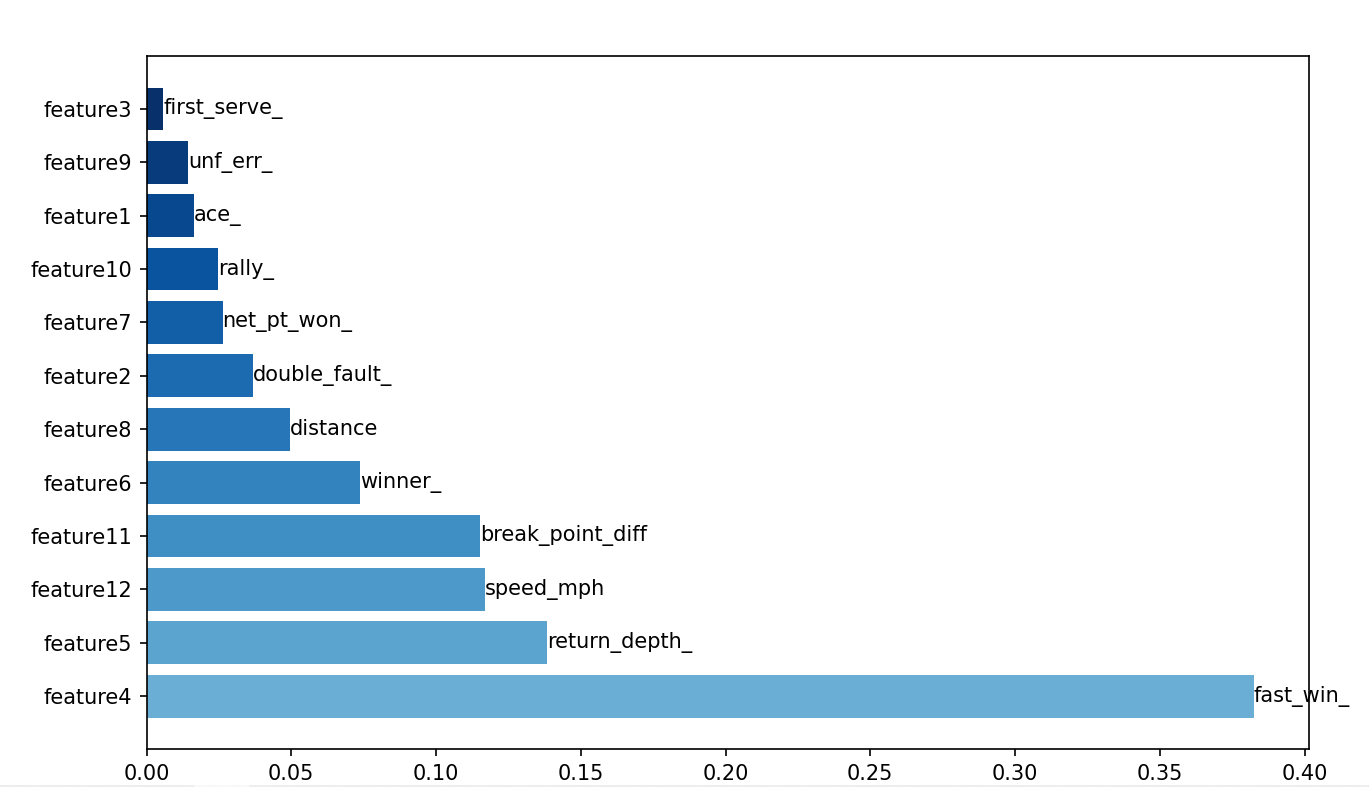
\includegraphics[scale=0.6]{mainmatter/imgs/8.png}
    \caption{feature importance}
\end{figure}

We can see that the most important feature is fast win(rally count < 3 and wins the point),
Because this time we only consider skill factors.this is related to our previous work,
%table of contents%%%%%%%%%%%%%%%%%%%
\tableofcontents 

%main matter%%%%%%%%%%%%%%%%%%%%%%%%%
\newpage
\setcounter{page}{1}
\rhead{Page \thepage\ }

\section{Introduction}

test

\subsection{Overview}

test

\subsection{Restatement of the Problem}

\paragraph{First Problem}

Momentum is “strength or force gained by motion or by a series of 
events.”It directly shows the player's current performance.
To assess the players' performance, it is crucial to have a clear understanding of ``momentum.'' 
We will focus on the following tasks: 
\begin{itemize}
    \item determine the influencing factors of ``momentum''
    \item Quantify the variations in ``momentum'' .
    \item Visualize the process of ``momentum'' changes.
\end{itemize}

\paragraph{Second Problem}

``momentum's role in the match'' means the level of momentum affects the future scores of the match.
The coach may subscribe to the idea that each point is an independent event and governed by probability.
In this view, consecutive success and momentum changes (swings) are seen as more random than influenced by previous events.
To judge this autocorrelation and to use our model, we 

\begin{itemize}
    \item perform autocorrelation test on momentum
    \item perform correlation test between current momentum and future scores.
\end{itemize}



\subsection{Assumptions}

To simplify the problem, we made the following assumptions:

\begin{itemize}
    \item \textbf{Assumption 1:} The \verb|px_unf_err| column of the data only counts those unforced errors that occurred when the player was hitting in baseline.\\
    \textbf{Justification:} Usually when a player is at net, the point will end in a few strikes, and there's little probability that the player will hit an unforced error within that few strikes. What's more, the \verb|px_net_point| and \verb|px_net_point_won| columns of the data can predominantly reflect the player's ability at net, therefore reducing the impact of counting the unforced errors while at net.
    
    \item \textbf{Assumption 2:} The current performance on a certain aspect of a player can be reflected by the player's 3 latest shots of that aspect.\\
    E.g. $P_{ace}$ can be reflected by the proportion of aces in the 3 latest \textbf{serves} of the player, $P_{win}$ can be reflected by the proportion of winners in the 3 latest \textbf{shots} of the player, $rd$ can be reflected by the return depth of the 3 latest \textbf{returns} of the player, etc. \\
    \textbf{Justification:} The current performance of a player consists of the average performance and the status of the player at the moment, which can be comprehensively reflected in the player's performance on recent shots. For convenience, we specified that the 3 latest shots can reflect the player's current performance.
\end{itemize}

\subsection{Our Work}

\begin{itemize}
    \item develop a model to 
\end{itemize}

\section{Momentum Evaluation Model}

\subsection{Model Introduction}~{}

To determine which player is performing better at a specific time, we create an indicator ``Momentum'' 
using the Analytic Hierarchy Process (AHP) \cite{AHP}to give a quantitative and overall evaluation.

\indent To investigate the reasons behind ``momentum'', we first need to provide a preliminary definition for ``momentum''. The magnitude of ``momentum'' is defined as 
$$M=\boldsymbol{\omega}\cdot\boldsymbol{x}$$
where:
\begin{enumerate}
    \item $M$ represents the ``momentum''.
    \item $\boldsymbol{x}$ is an $n$-dimensional column vector representing some influencing factors. Specific details will be provided later.
    \item $\boldsymbol{\omega}$ is an $n$-dimensional row vector indicating the specific weights of the influencing factors, which will be obtained through the Analytic Hierarchy Process (AHP).
    \item In this formula, there are two different calculation situations, one representing rounds where the player serves and the other representing rounds where the opponent serves. We can express it as $$\boldsymbol{\omega}=\boldsymbol{\omega_0} \circ \boldsymbol{\delta}=(\omega_0^{(0)}\delta^{(0)},\omega_0^{(1)}\delta^{(1)},\dots,\omega_0^{(n)}\delta^{(n)})$$  Here, $\boldsymbol{\delta}$ is a $0,1$ vector indicating whether it is the player's serving round. In the specific calculation, we will consider two cases separately.
\end{enumerate}

Out of our own interpretation of AHP, we will break down the problems into three parts:

\begin{enumerate}
    \item Factor Normalization and Data Cleaning
    \item Collinearity Detection
    \item Analytic Hierarchy Process (AHP)
\end{enumerate}

\subsubsection{Notations}~{}

\begin{table}[H]
\centering
\begin{tabular}{cccccc}
    
    \toprule
    Symbols & Description \\ 
    \midrule
    $player$ & the current player we are considering (e.g. while calculating momentum) \\
    $point_i$ & the $i^{th}$ point of the match, a vector consists of fields stated in the given dictionary \\
    $cur$ & the current index of the point, i.e. the match is currently at the $cur^{th}$ point \\
    $H_i$ & denotes the set $\{point_{cur}, point_{cur - 1}, \ldots , point_{cur - i + 1}\}$ \\
    $S_i$ & the set of latest $i$ points where $player$ serves\\
    $R_i$ & the set of latest $i$ points where $player$ returns\\
    $P_{ace}$ & current probability of hitting an ace by $player$ \\
    $P_{df}$ & current probability of double-faulting by $player$ \\
    $P_{1st}$ & current first serve goal rate by $player$ \\
    $P_{fw}$ & current probability of $player$ winning a served point within 3 rallies \\
    $rd$ & current return depth of $player$ \\
    $P_{win}$ & current probability of hitting a winner by $player$ \\
    $P_{net}$ & current net win rate of $player$ \\
    $dist$ & $player$'s running distance on the point \\
    $P_{unf}$ & current probability of hitting an unforced error by $player$ \\
    $scored$ & whether $player$ scored the current point \\
    $diff$ & the score diffrence for $player$ in the current game (by number of points) \\
    $M$ & the current momentum of $player$ after a point \\

    \bottomrule
\end{tabular}
\end{table}
To access a certain field in a point, we simply use the field name stated in the given 
dictionary as index, i.e. for a point $point$, we use $point_{ace}$ to denote the binary 
variable that shows whether $player$ hits an ace ball in the point.


\subsubsection{Factor Normalization and Data Cleaning}~{}

For the specific definition of $\boldsymbol{x}$, we believe that, 
in addition to whether the player is serving, many other factors can have an impact,
including the player's skills, fatigue level, and real-time mental state of the games.
Based on these three main aspects, 
we have organized 12 factors as preliminary influencing factors, as follows:

\begin{equation}
    P_{ace} = \frac{\sum_{p \in S_3} p_{ace}}{3}
\end{equation}
\begin{equation}
    P_{df} = -\frac{\sum_{p \in S_3} p_{double\_fault}}{3}
\end{equation}
\begin{equation}
    P_{1st} = \frac{\sum_{p \in S_3} [p_{serve\_no} = 1]}{3}
\end{equation}
\begin{equation}
    P_{fw} = \frac{\sum_{p \in S_3} [p_{rally\_count} \le 3] [p_{point\_victor} = player]}{3}
\end{equation}
\begin{equation}
    rd = \frac{\sum_{p \in R_3} \left\{
        \begin{aligned}
        0, && p_{return\_depth} = ND \\
        1, && p_{return\_depth} = D \\
        -1, && p_{return\_depth} = NA \\
        \end{aligned}
        \right.}{3}
\end{equation}
\begin{equation}
    P_{win} = \frac{\sum_{p \in H_3} p_{winner}}{3}
\end{equation}
\begin{equation}
    P_{net} = \frac{\sum_{p \in H_3} p_{net\_pt\_won}}{\sum_{p \in H_3} p_{net\_pt}}
\end{equation}
\begin{equation}
    dist = \left\{
        \begin{aligned}
        0, && point_{cur, distance\_run} < 5 \\
        -1, && point_{cur, distance\_run} > 45 \\
        \frac{5 - point_{cur, distance\_run}}{40}, && otherwise \\
        \end{aligned}
        \right.
\end{equation}
\begin{equation}
    P_{unf} = -\frac{\sum_{p \in H_3} p_{unf\_err}}{3}
\end{equation}
\begin{equation}
    scored = [point_{cur, point\_victor} = player]
\end{equation}
\begin{equation}
    diff = \frac{\sum_{p \in point}[p_{set\_no} = point_{cur, set\_no}][p_{game\_no} = point_{cur, game\_no}](2[p_{point\_victor} = player]-1)}{\min\{3, \sum_{p \in point}[p_{set\_no} = point_{cur, set\_no}][p_{game\_no} = point_{cur, game\_no}]\}}
\end{equation}

\par In order to normalize the data processed, we convert the original data to limit them in $[-1, 1]$. 
For those factors that negatively influence the momentum, such as $P_{df}$, we made sure it's in $[-1, 0]$. For those factors that positively influence the momentum, such as $P_{win}$, we made sure it's in $[0, 1]$. For those factors that influence the momentum in both ways, such as $diff$, we made sure it's in $[-1, 1]$.

\subsubsection{Collinearity Detection}~{}

After data processing, considering the potential collinearity among factors within the same category,
such as serving aces, first-serve scoring rate, and whether the previous point was scored may 
be correlated, as well as running distance and the number of strokes possibly being related, 
we conduct collinearity detection using Stata. The results of the detection indicate a
significant variance inflation factor between running distance and the number of strokes. 
Therefore, we decided to exclude one of them, choosing to retain the remaining 11 variables 
for the Analytic Hierarchy Process (AHP), as follows:

\begin{figure}[H]
    \centering
    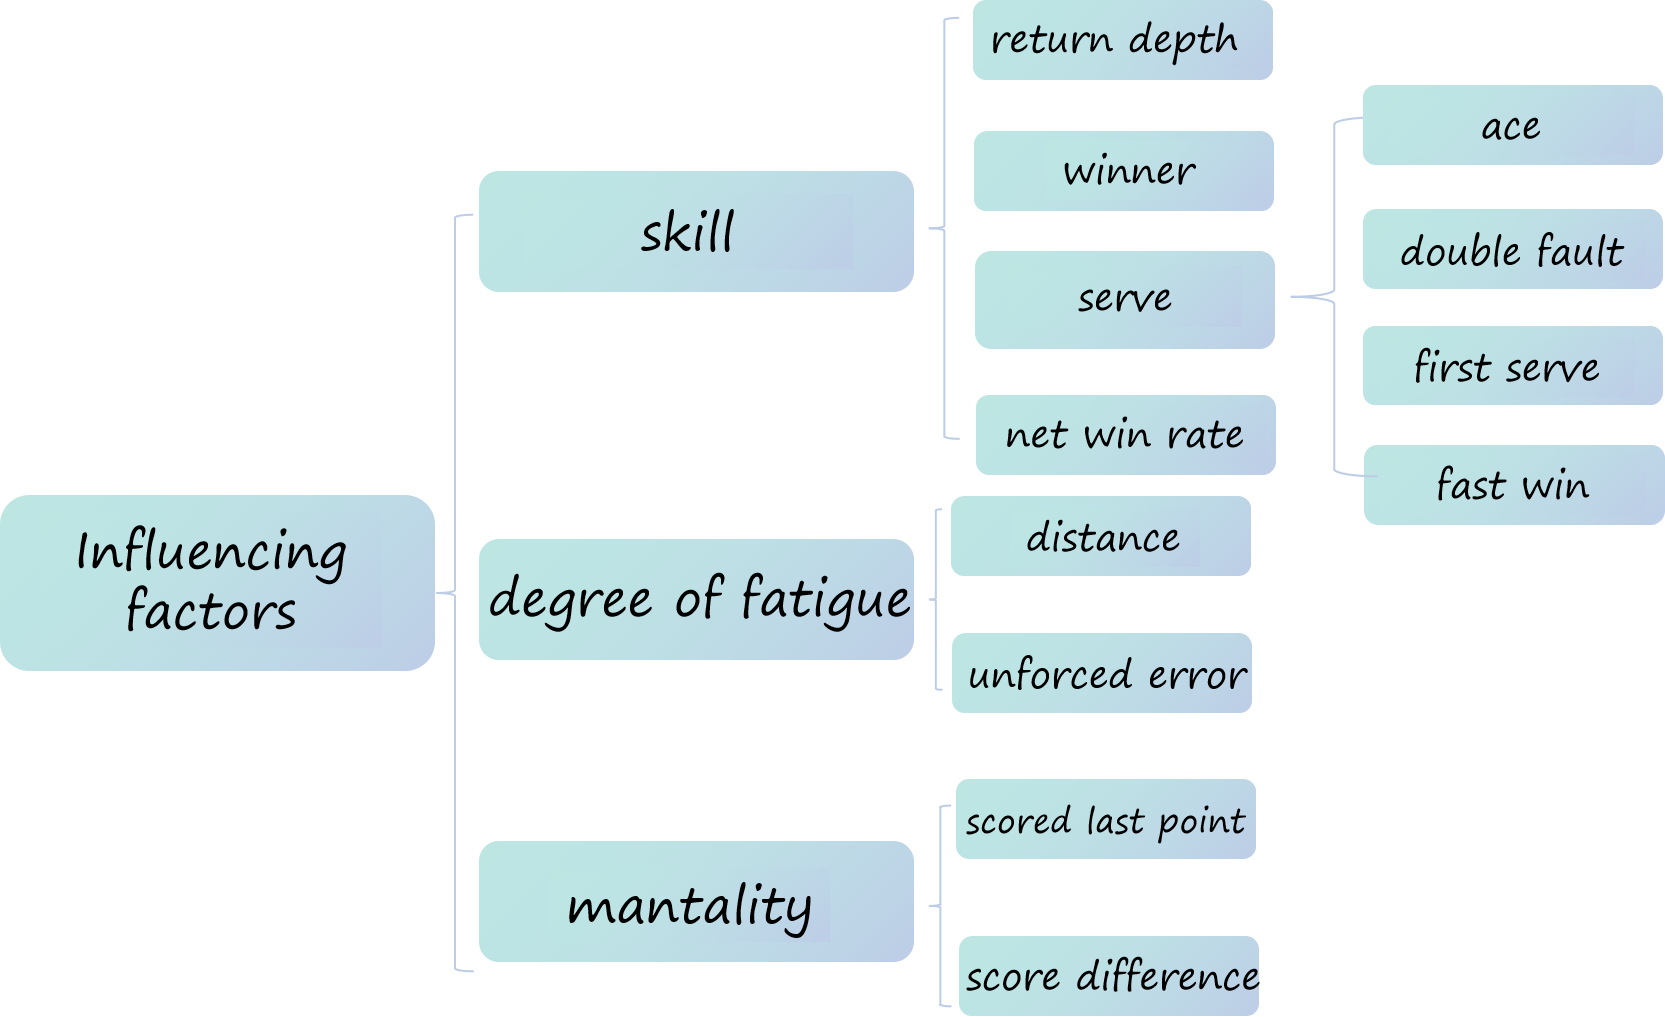
\includegraphics[width=0.6\textwidth]{mainmatter/imgs/11.png}
    \caption{Non-collinear factors}
    \label{fig:11var}
\end{figure}


\subsubsection{Analytic Hierarchy Process}~{}

We have previously decomposed the included factors from top to bottom into several levels, 
where factors within the same level are subordinate to factors in the level above or influence 
factors in the level above. They also dominate factors in the next level or are influenced by 
factors in the next level. Starting from the second level of the hierarchy, we construct 
comparison matrices for each factor influencing the factor in the level above, until reaching 
the bottom level. Each element in the matrix indicates the preference level between factor i and 
factor j at the same level. It is essential to note that we have separately established a series 
of such comparison matrices for two different serving types (serve by oneself and serve by 
the opponent). Here, we illustrate the matrix using serve by oneself as an example:

\begin{figure}[H]
    \centering
    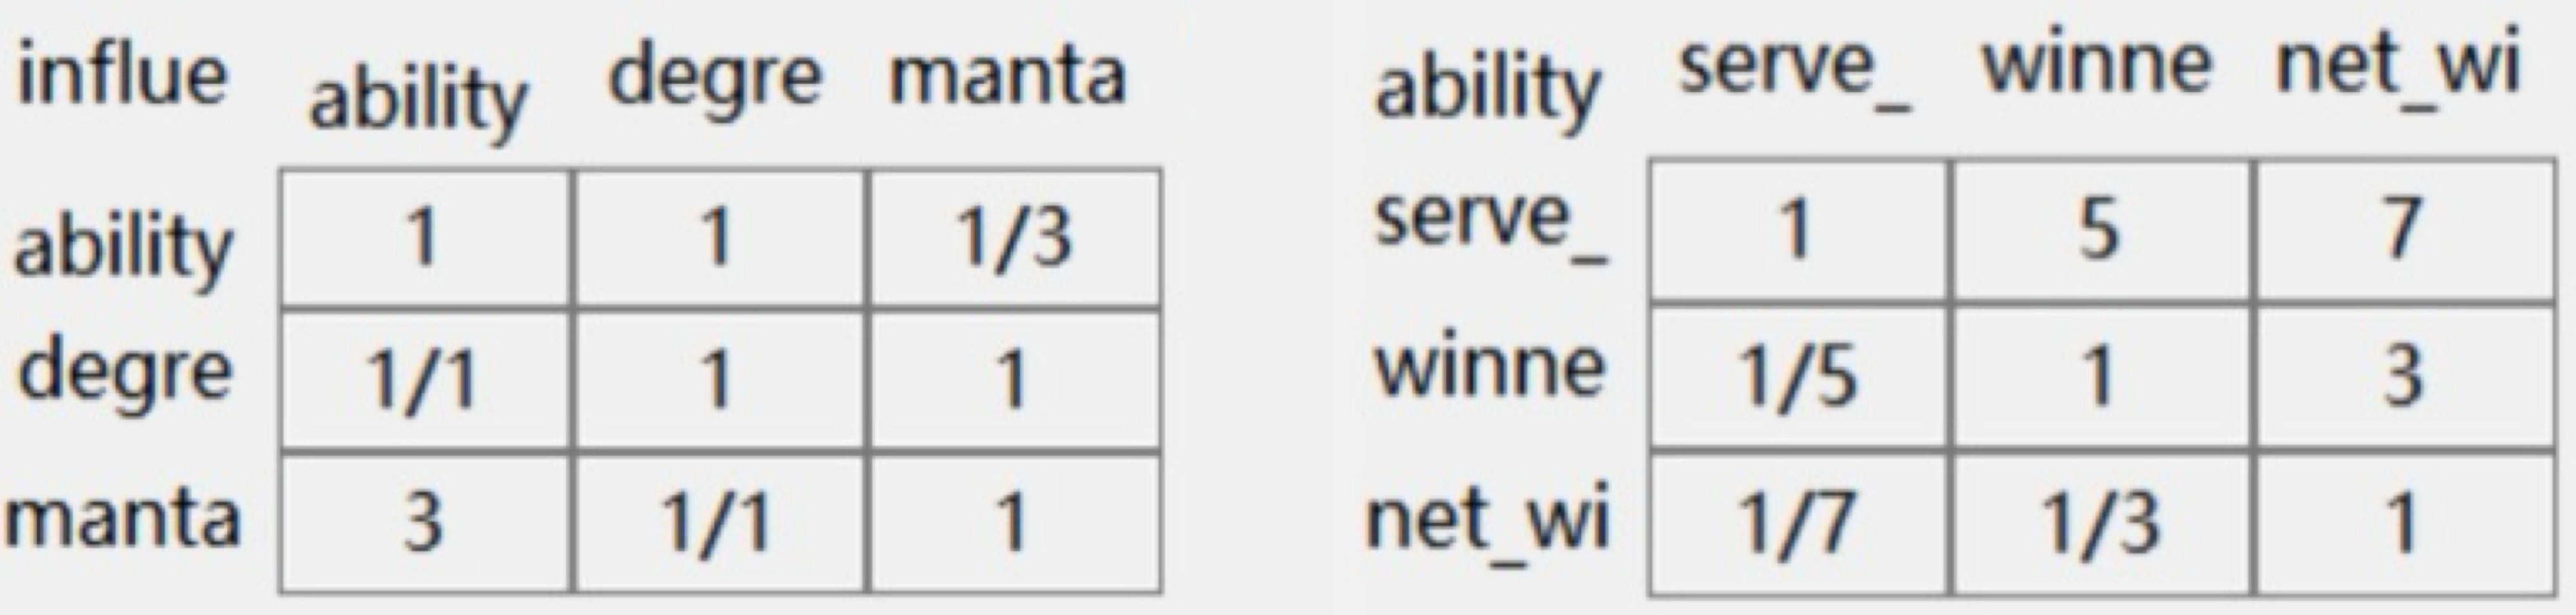
\includegraphics[scale=0.06]{mainmatter/imgs/2.jpg}
    \caption{Comparison matrix for influencing factors and ability}
\end{figure}
\begin{figure}[H]
    \centering
    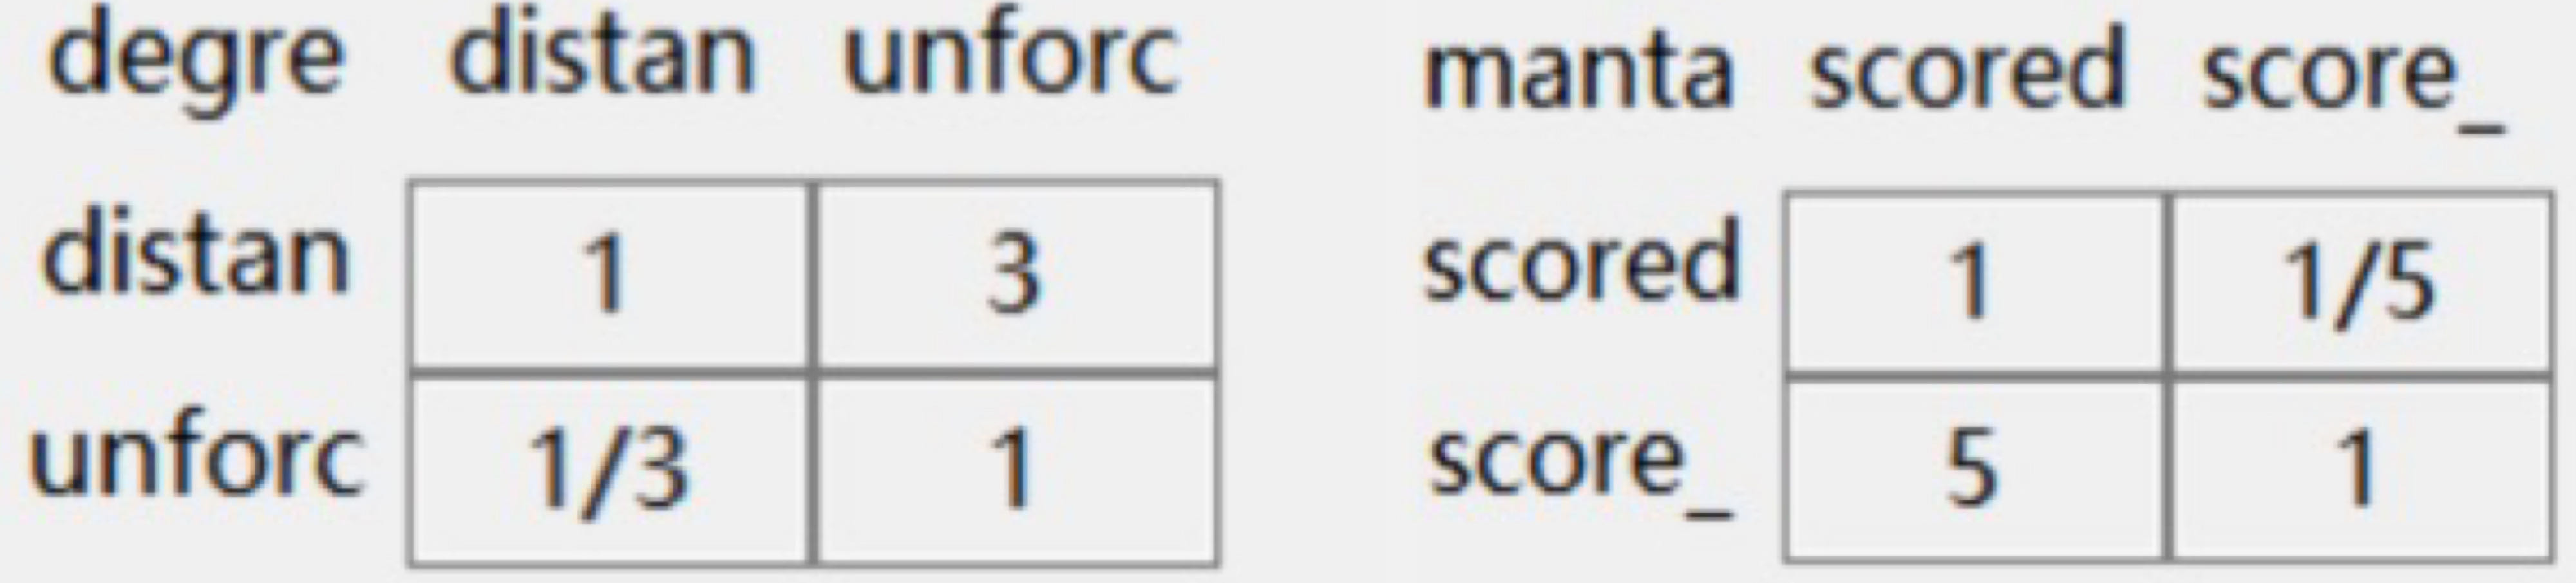
\includegraphics[scale=0.05]{mainmatter/imgs/3.jpg}
    \caption{Comparison matrix for degree of fatigue and mantality}
\end{figure}
\begin{figure}[H]
    \centering
    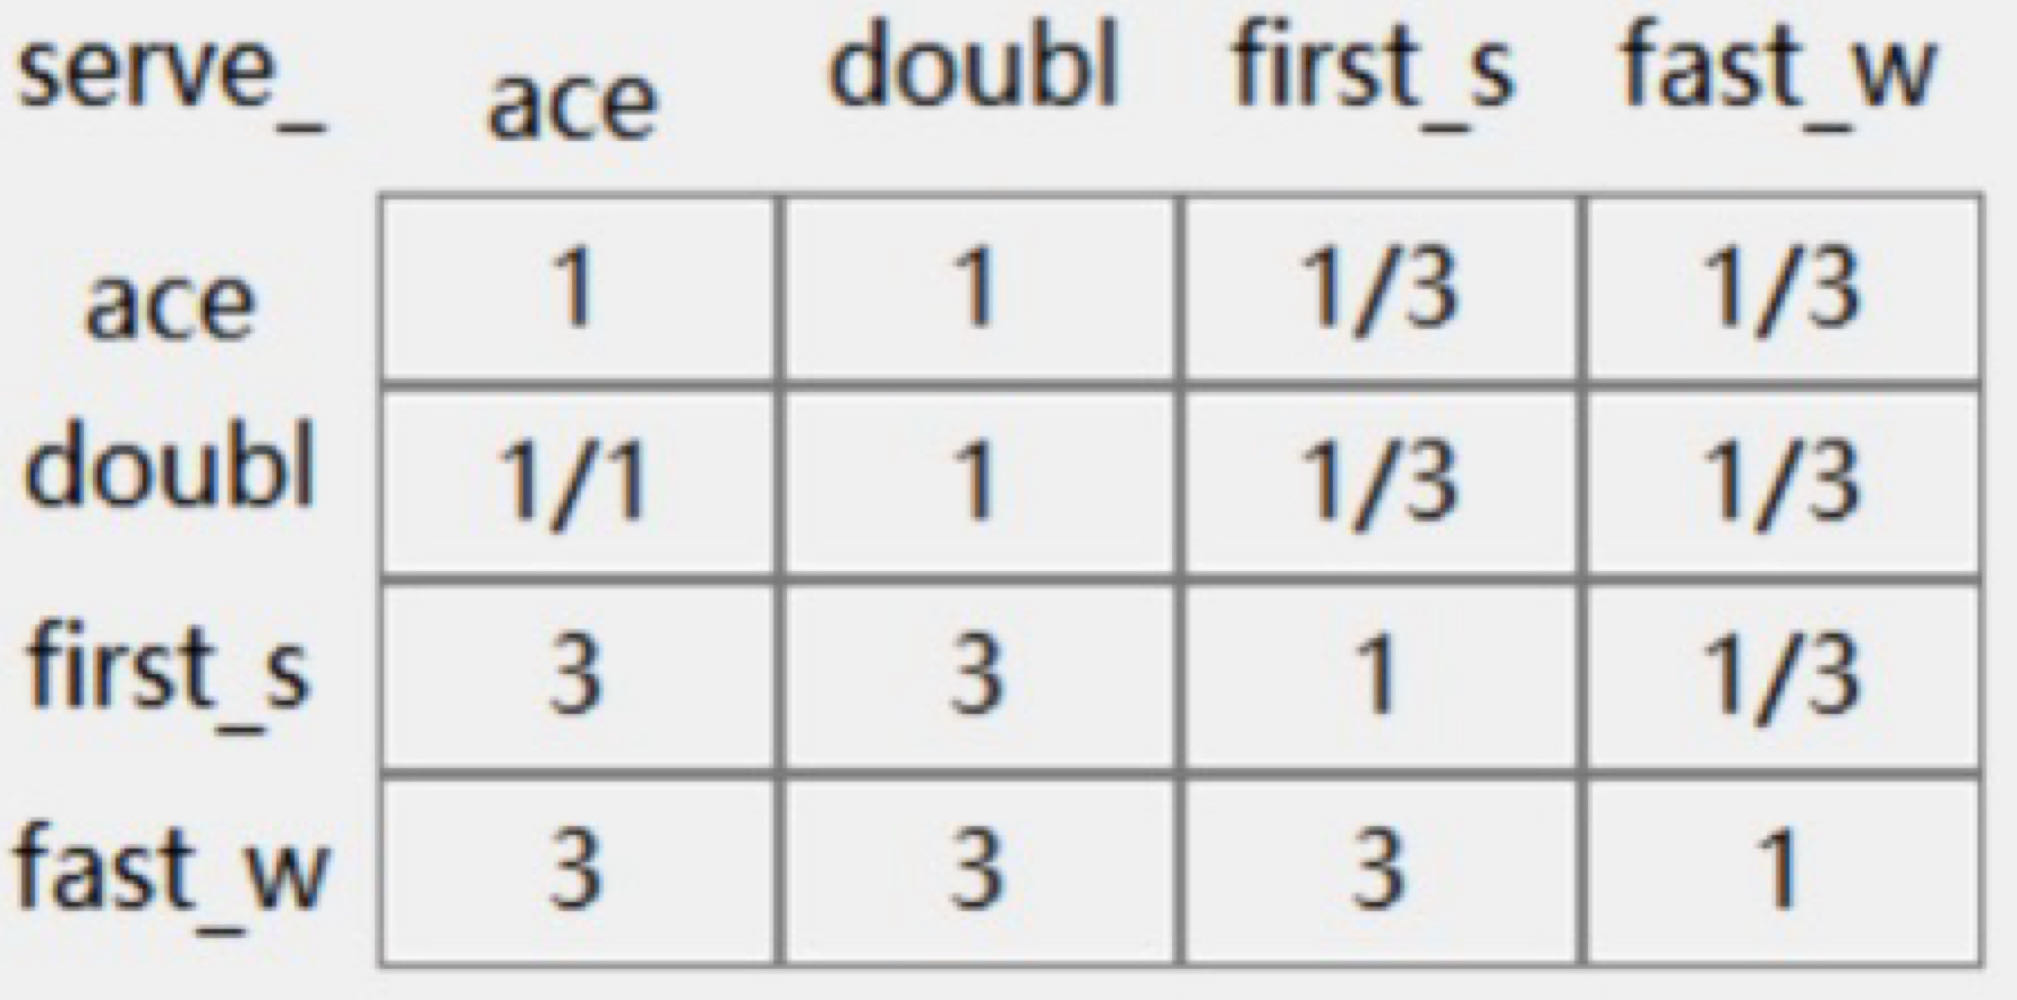
\includegraphics[scale=0.06]{mainmatter/imgs/4.jpg}
    \caption{Comparison matrix for serving}
\end{figure}

We obtain the weights for each component by calculating the maximum eigenvalue and normalizing 
its corresponding eigenvector. Certainly, for each matrix, we first need to test consistency 
using the Consistency Ratio (CR), where \(CR=\frac{CI}{RI}\), \(CI=\frac{\lambda_{max}-n}{n-1}\), 
\(RI=0.0, 0.58, 0.9\) (for matrices of size \(2, 3, 4\)). The computed Consistency Ratios for the 
matrices are 0.076, 0.037, 0.0, 0.0, 0.046. Since they are all less than 0.1, it confirms the 
consistency of the matrices.\\

\indent Therefore, the weights for our model are as follows:


\begin{figure}[H]
    \centering
    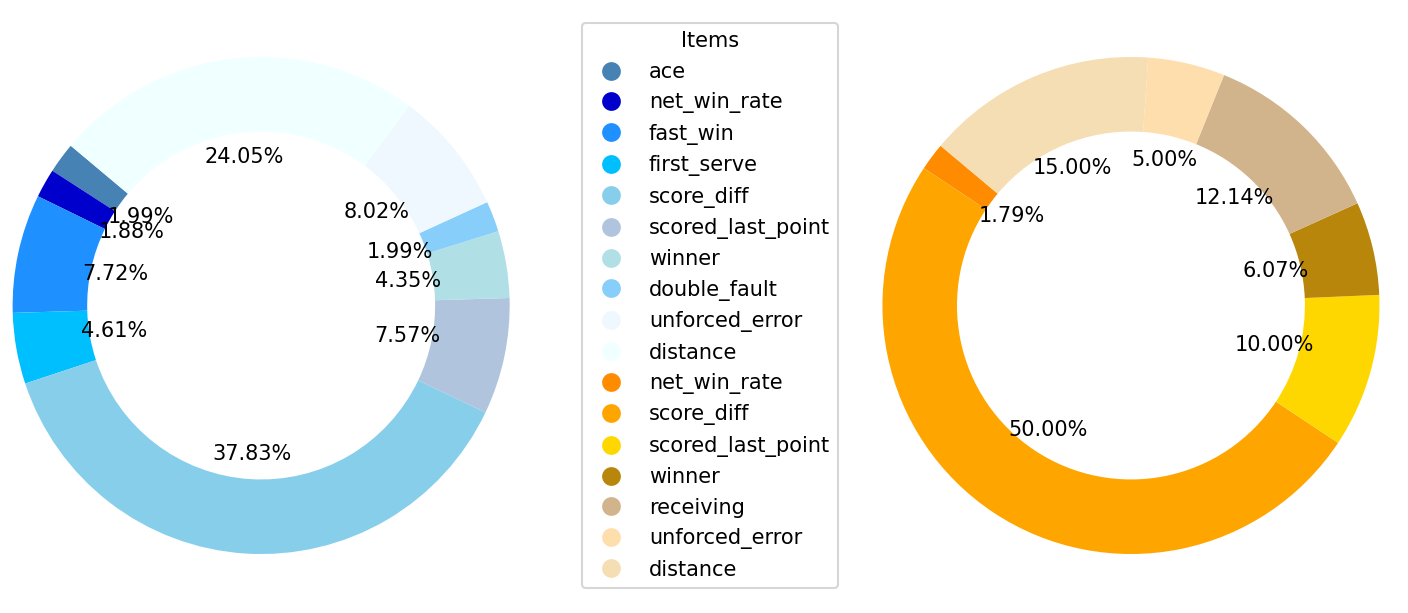
\includegraphics[scale=0.65]{mainmatter/imgs/7.png}
    \caption{Weights in two different situations}
\end{figure}

Analyzing the various factors in the chart, it is evident that the most impactful factor is 
whether the previous point was scored. Following closely is the distance covered during the 
play, which aligns well with common intuition.\\

Thus, our final momentum is defined as:
$$M=\begin{cases}
    \sum\limits_{n=1,n\neq 5}^{11}\omega_n x_n, & \text{if the player serves}  \\
    \sum\limits_{n=5}^{11}\omega_n x_n, & \text{if the opponent serves}
\end{cases}$$
Where $\omega_n(n=1,\dots,11)$ represent the weight of the factors, which is listed in Figure 4.\\

\subsection{Visualization and Analysis}~{}

Now, we illustrate the graph of the "momentum" in the first match:

\begin{figure}[H]
    \centering
    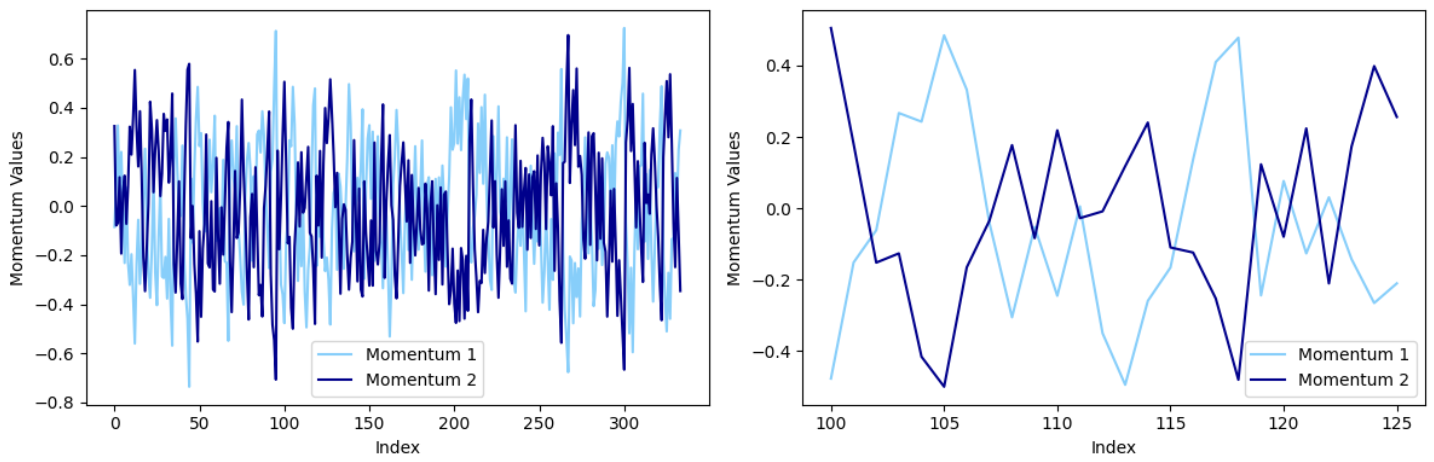
\includegraphics[scale=0.65]{mainmatter/imgs/5.png}
    \caption{Momentum change in the first competition(global and local)}
\end{figure}

It can be observed that the variation in ``momentum'' is a process of give and take.
When momentum 1 is higher than momentum 2, it means that the player 1 is performing better than the opponent. 

\subsection{momentum autocorrelation and correlation with runs of success}~{}

To answer the coach's doubt,
we need to perform autocorrelation test on momentum, 
and perform correlation test between current momentum and future scores
in this section.

If the momentum has a high autocorrelation, it means that the momentum at this moment 
has a high impact on future performance. And if the correlation between momentum and 
future scores is high, it means that the player with higher momentum has a higher
chance to win the next multiple round.

\subsubsection{momentum autocorrelation}~{}

To check if sequence of momentum is self-related, we calculate the Pearson correlation 
between momentum and that with a time lag.

\begin{algorithm}
    \caption{Calculate Autocorrelation Function}\label{alg:auto_corr}
    \begin{algorithmic}
        \For{$i = 1$ to $31$}
            \State $time\_series \gets \text{momentum}(i^{th}\ \text{match\_index} : {i+1}^{th}\ \text{match\_index} - 1)$
            \State $max\_lag \gets \lfloor \text{length}(time\_series) / 2 \rfloor$ \Comment{Consider lags up to half of the length of the time series}
            \State $autocorrelation \gets \text{zeros}(1, max\_lag)$

            \For{$shift = 1$ to $max\_lag$}
                \State $correlation \gets \text{corrcoef}(time\_series(1 : \text{end} - shift), time\_series(shift + 1 : \text{end}))$
                \State $autocorrelation(shift) \gets correlation(1, 2)$
            \EndFor

            \Comment{Further processing or visualization can be performed here}
        \EndFor
    \end{algorithmic}
\end{algorithm}

Here we display the autocorrelation of momentum of the first player in first three games.
There are similar results for the second player and for the momentum difference.

\begin{figure}[H]
    \centering
    \begin{subfigure}[b]{0.34\textwidth}
        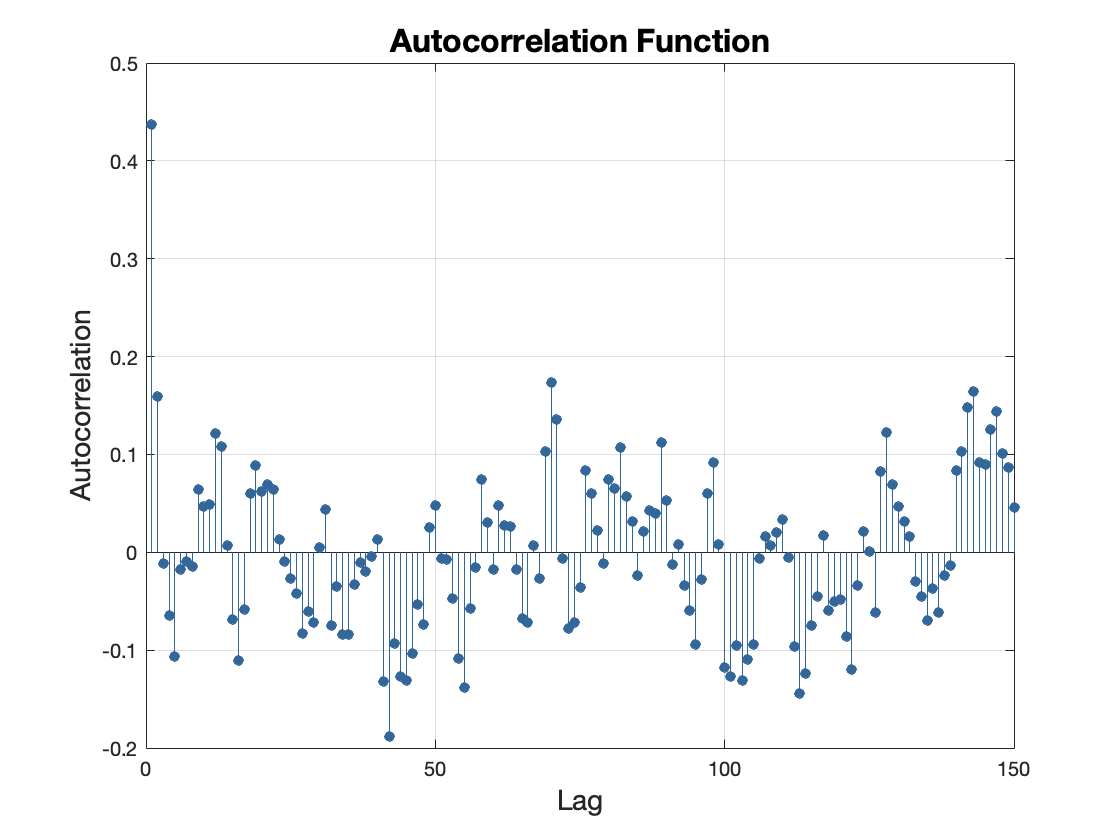
\includegraphics[width=\linewidth]{mainmatter/imgs/momen_selfco_1.png}
        \caption{autocorrelation in match 1}
    \end{subfigure}\hspace{-0.02\textwidth}
    \begin{subfigure}[b]{0.34\textwidth}
        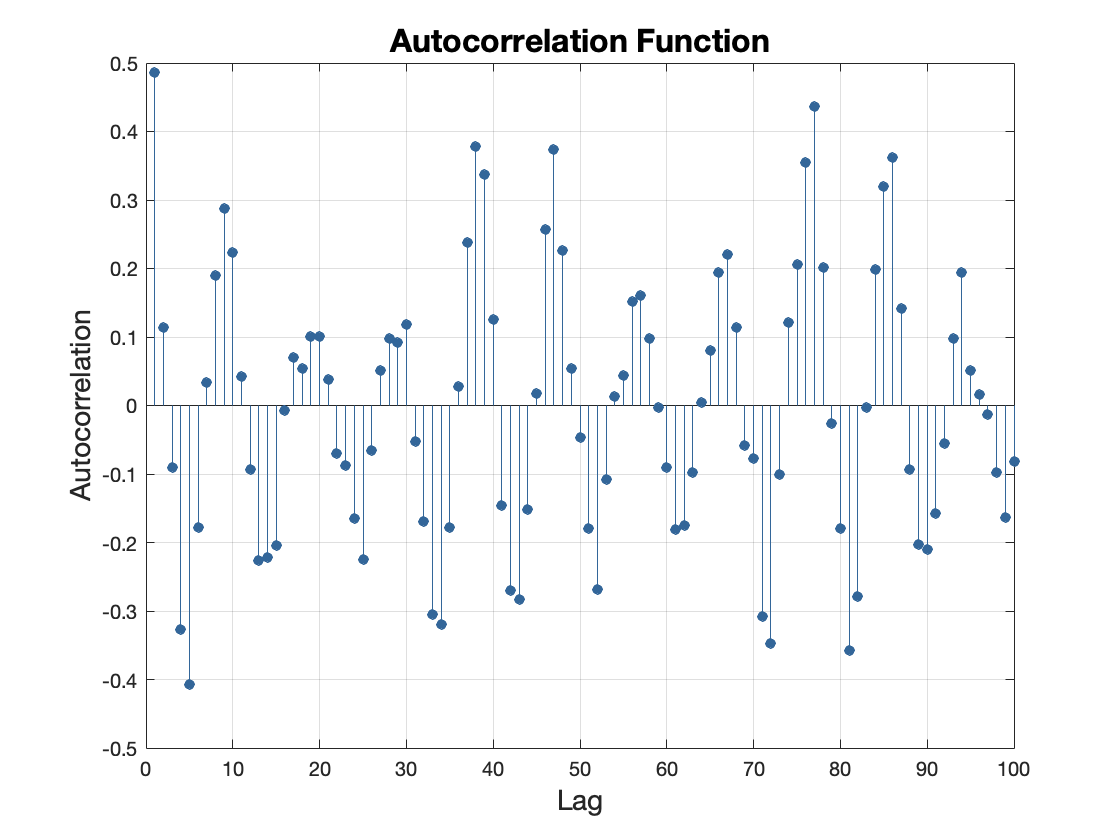
\includegraphics[width=\linewidth]{mainmatter/imgs/momen_selfco_2.png}
        \caption{autocorrelation in match 2}
    \end{subfigure}\hspace{-0.02\textwidth}
    \begin{subfigure}[b]{0.34\textwidth}
        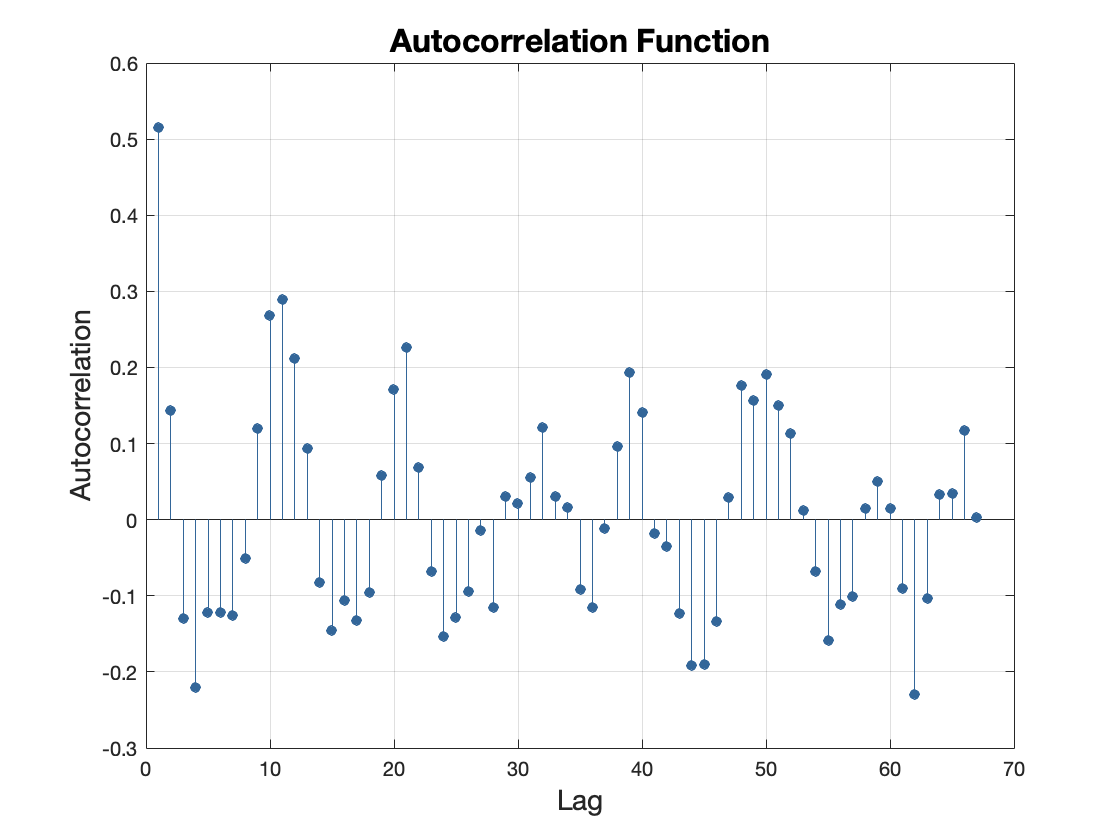
\includegraphics[width=\linewidth]{mainmatter/imgs/momen_selfco_3.png}
        \caption{autocorrelation in match 3}
    \end{subfigure}
    \caption{Momentum autocorrelation}
    \label{fig:Correlation}
\end{figure}

The corrcoef of lag 1 in match one is 0.4546, match two 0.5149,match three 0.5342.
It can be seen that the autocorrelation of lag one is high, which means that the momentum at this moment
has a strong relationship with the momentum in the next round. And the autocorrelation decreases to random 
as the lag increases.

\subsubsection{correlation with runs of success}~{}

To give a quantitative evaluation of ``future scores'', we count points gain in future multiple rounds,
and derive the difference by minus that of the opponent. 
For example, if the player gains 3 points in the next 5 rounds, and the opponent gains 2 points,
the difference is 1.
The difference indicates how much better the player is performing than the opponent.

In intuition, the player with higher momentum should have a higher chance to win the next round.
And momentum at this moment should have less impact on the future rounds as time extends.
The correlation between momentum and future scores verifies our intuition.

We calculate points gain difference in future one to five rounds at each time of all matches.
Here we display five points gain difference and momentum difference in first three games.

\begin{figure}[H]
    \centering
    \begin{subfigure}[b]{0.34\textwidth}
        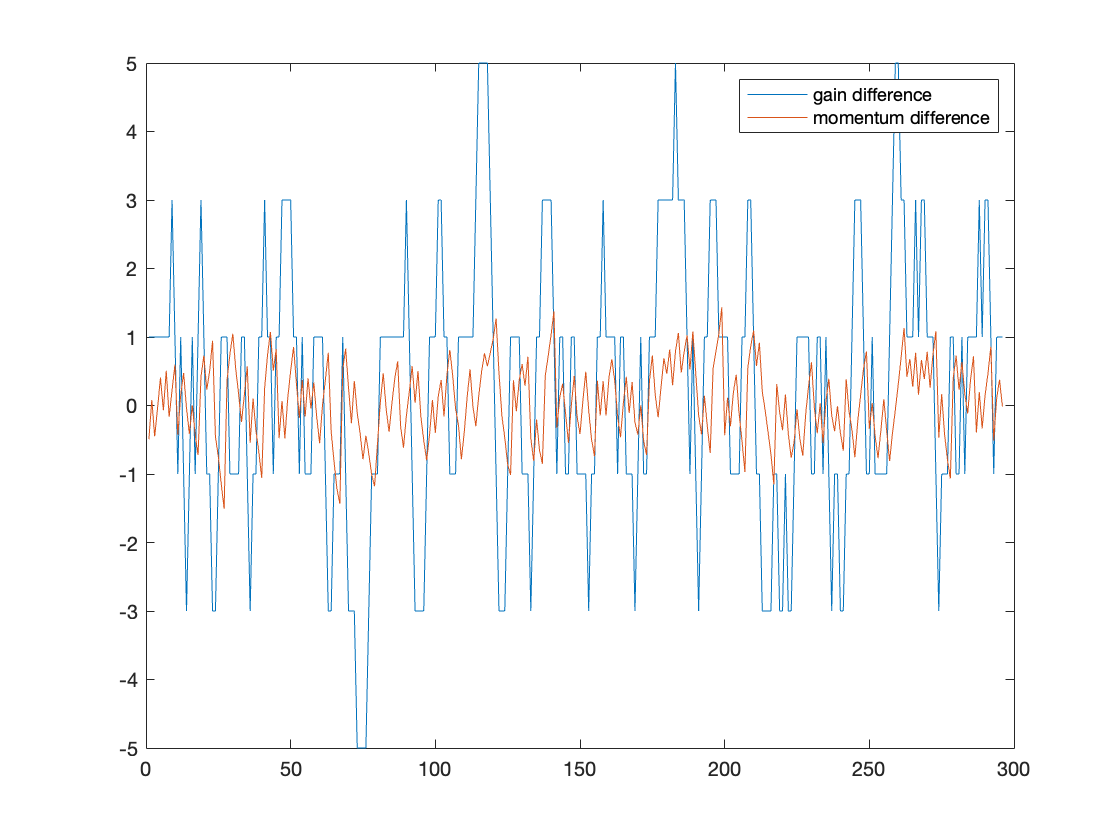
\includegraphics[width=\linewidth]{mainmatter/imgs/diff_match1.png}
        \caption{2023-wimbledon-1301}
    \end{subfigure}\hspace{-0.02\textwidth}
    \begin{subfigure}[b]{0.34\textwidth}
        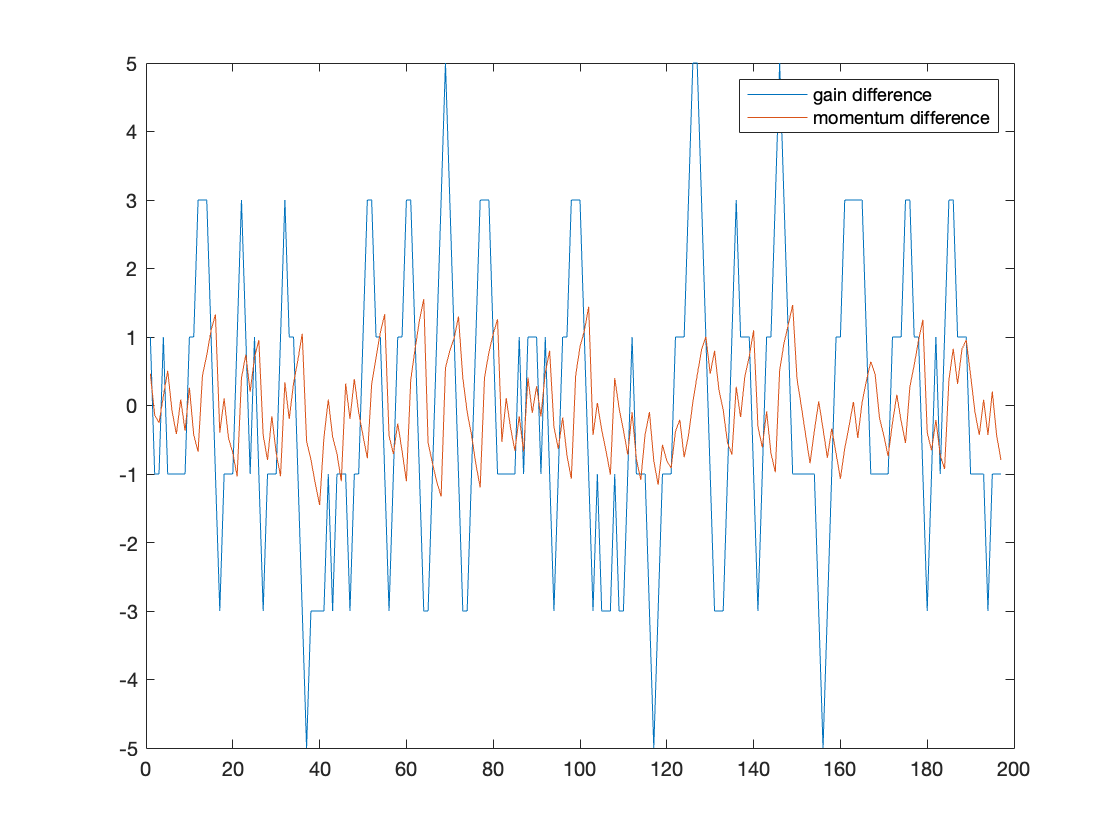
\includegraphics[width=\linewidth]{mainmatter/imgs/diff_match2.png}
        \caption{2023-wimbledon-1302}
    \end{subfigure}\hspace{-0.02\textwidth}
    \begin{subfigure}[b]{0.34\textwidth}
        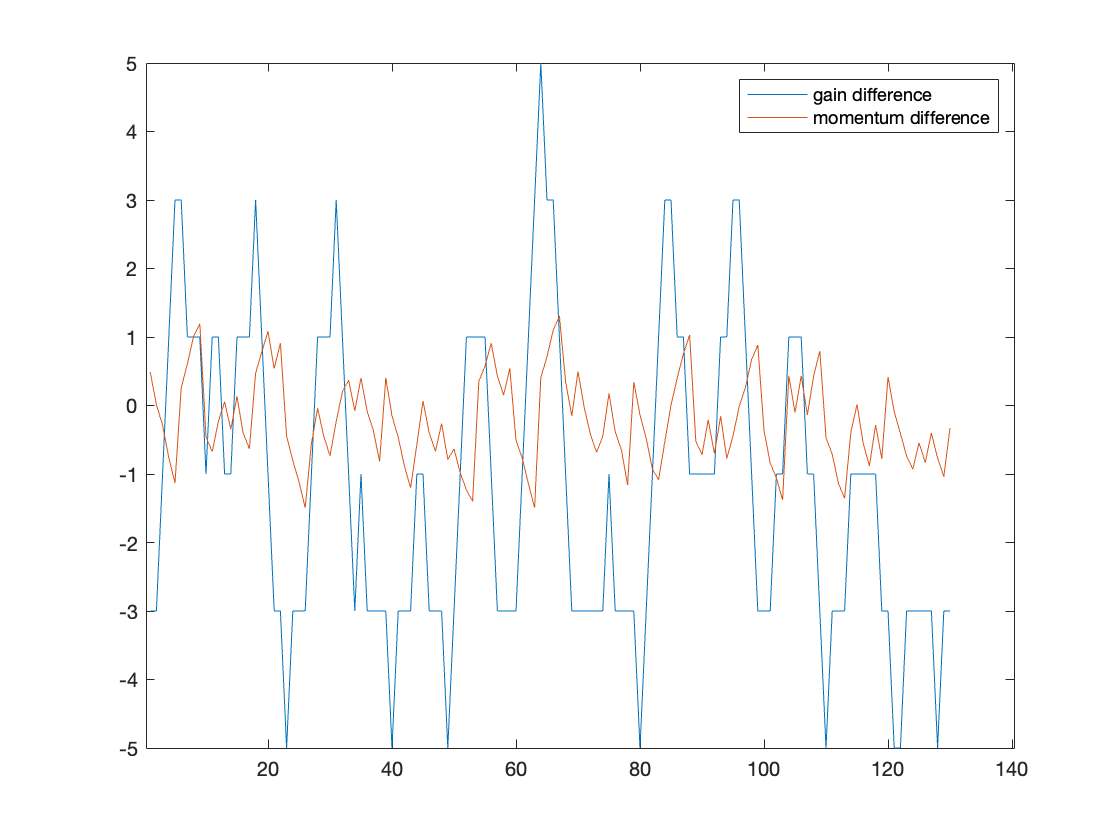
\includegraphics[width=\linewidth]{mainmatter/imgs/diff_match3.png}
        \caption{2023-wimbledon-1303}
    \end{subfigure}
    \caption{Gain Difference and Momentum in First Three Games}
    \label{fig:Gain Difference and Momentum}
\end{figure}

And we derive the correlation between gain difference from one to five rounds 
and momentum difference of all matches. Here we display the three of them.

\begin{figure}[H]
    \centering
    \begin{subfigure}[b]{0.34\textwidth}
        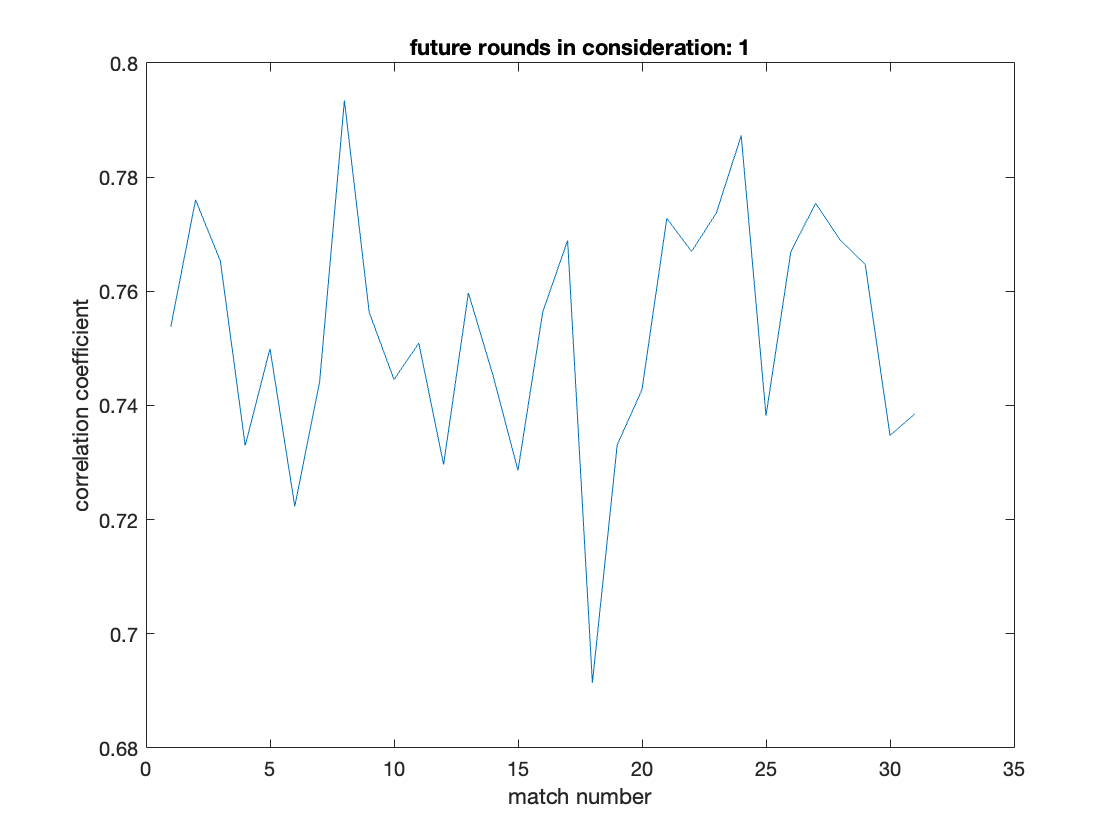
\includegraphics[width=\linewidth]{mainmatter/imgs/momen_1points_cor.png}
        \caption{gain difference in 1 round}
    \end{subfigure}\hspace{-0.02\textwidth}
    \begin{subfigure}[b]{0.34\textwidth}
        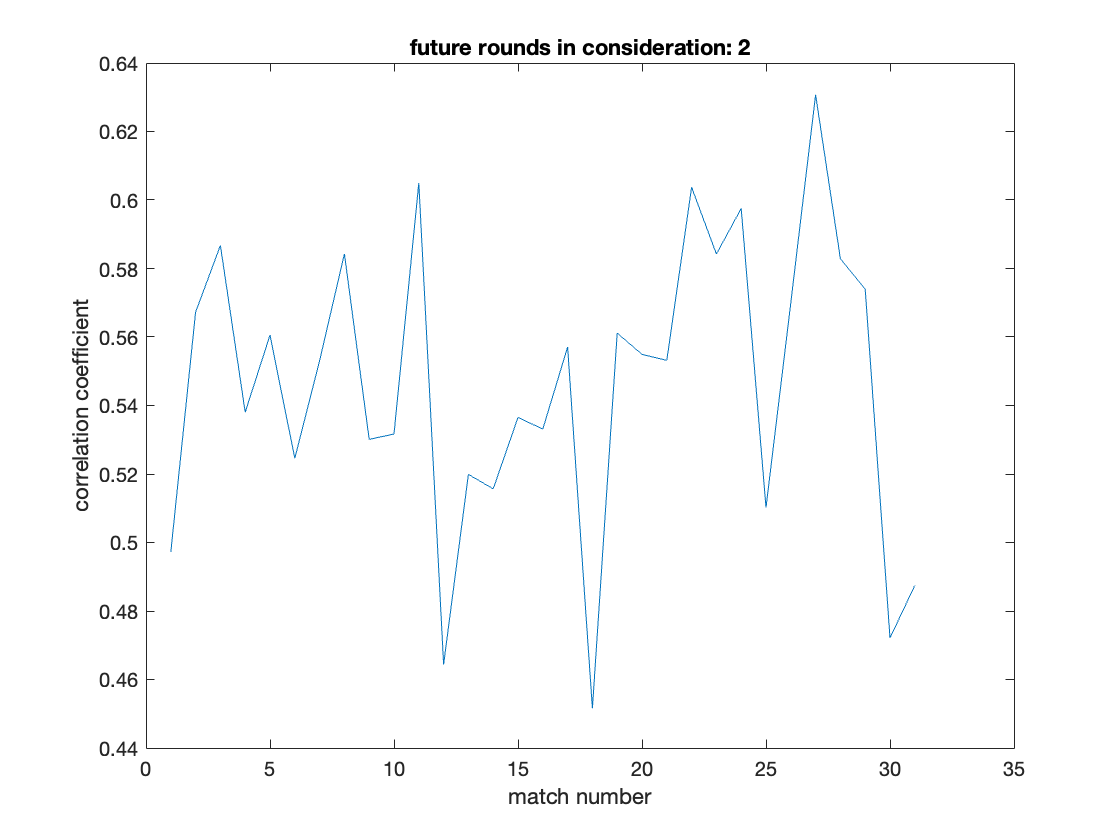
\includegraphics[width=\linewidth]{mainmatter/imgs/momen_2points_cor.png}
        \caption{gain difference in 2 rounds}
    \end{subfigure}\hspace{-0.02\textwidth}
    \begin{subfigure}[b]{0.34\textwidth}
        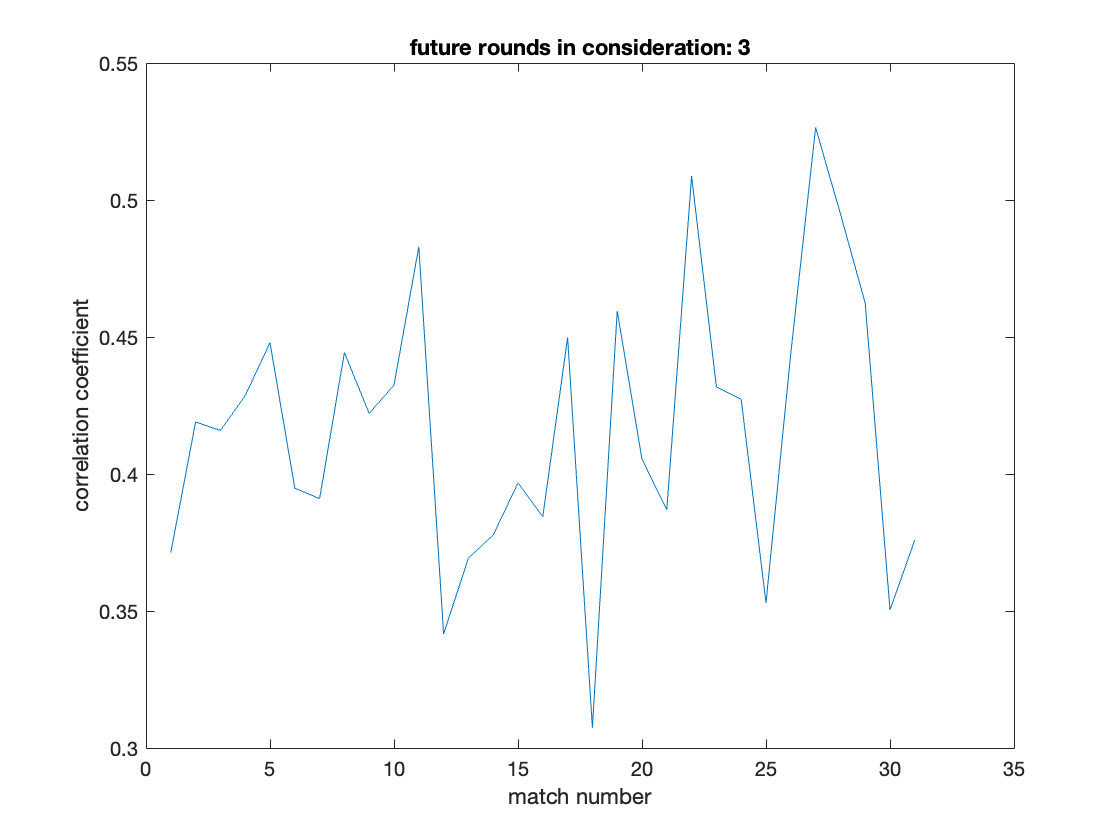
\includegraphics[width=\linewidth]{mainmatter/imgs/momen_3points_cor.png}
        \caption{gain difference in 3 rounds}
    \end{subfigure}
    \caption{Correlation Between Gain Difference and Momentum Difference}
    \label{fig:Correlation}
\end{figure}

Here we display the max and min correlation in different rounds.
(hint. the max and min correlation means maximum and minimum of all matches.)

\begin{table}[H]
    \centering
    \begin{tabular}{ccccccc}
        \toprule
        \textbf{Rounds} & \textbf{1} & \textbf{2} & \textbf{3} & \textbf{4} & \textbf{5} \\
        \midrule
        \textbf{Max} & 0.7934 & 0.6307 & 0.5264 & 0.4678 & 0.3910 \\
        \textbf{Min} & 0.6914 & 0.4516 & 0.3074 & 0.1824 & 0.0627 \\
        \bottomrule
    \end{tabular}
    \caption{Maximum and Minimum Correlation of all matches in different rounds}
    \label{fig:maxmin_correlation}
\end{table}

As we can see from the table, the correlation between momentum and future scores is bigger
than 0.5 considering the next 1 round, it implies that momentum has a substantial impact on the next round.
And the correlation decreases as the rounds extend, which verifies our intuition, that
the momentum at this moment has less impact on the future rounds as time extends.

Now, we have finished problem 1 and 2.

\section{Swing Prediction Model}

\subsection{Model Introduction}~{}

To predict the swings, we need to find potential factors that may affect future momentum.
In problem 1, we established a standard to judge the player's performance;
in problem 2, we found the player's performance, ``momentum'', has a one order of autocorrelation,
which indicates that some factors of the momentum have impact on the future momentum.

To find what and how factors affect the future momentum, we can take advantage 
of Machine Learning. In this section, we will primarily focus on establishing a 
supervised learning classification model using the Gated Recurrent Unit (GRU) network to 
predict momentum swings. We will break down the problems into three parts:

\begin{itemize}
    \item definition of the swing of the play
    \item data (potential factors) and label used to train GRU
    \item Utilizing Gated Recurrent Unit
\end{itemize}

\subsubsection{Definition of ``Swings of the Play''}~{}

We first give the definition of the swings of the play.
Based on our previous definition of ``momentum,'' the significant changes of the game 
largely depend on the ``momentum'' of the two players. Therefore, we choose ``momentum'' to represent 
the swings of the play. The specific definition is as follows:\\

We use $\Delta f(t)$ to represent the difference in ``momentum'' between the two players., 
so it can be easily seen that if $\Delta f(t)$ and $\Delta f(t+1)$
have different signs, it indicates a ``swing'' in the game's momentum. 
In this way, we can define four states of ``momentum'' at time $t$:

$$states=\begin{cases}
    state1, &\text{if } \Delta f(t)>0 \text{ and } \Delta f(t+1)>0, \text{ which means stay positive}\\
    state2, &\text{if } \Delta f(t)<0 \text{ and } \Delta f(t+1)>0, \text{ which means rise from negative to positive}\\
    state3, &\text{if } \Delta f(t)<0 \text{ and } \Delta f(t+1)<0, \text{ which means stay negative}\\
    state4, &\text{if } \Delta f(t)>0 \text{ and } \Delta f(t+1)<0, \text{ which means decrease from positive to negative}
\end{cases}$$
Obviously, if state 2 or state 4 appears, we can determine that a swing has occurred. 

To visualize the swing, we choose four shapes of lines to represent the four states of swings at time $t$:

\begin{figure}[H]
    \centering
        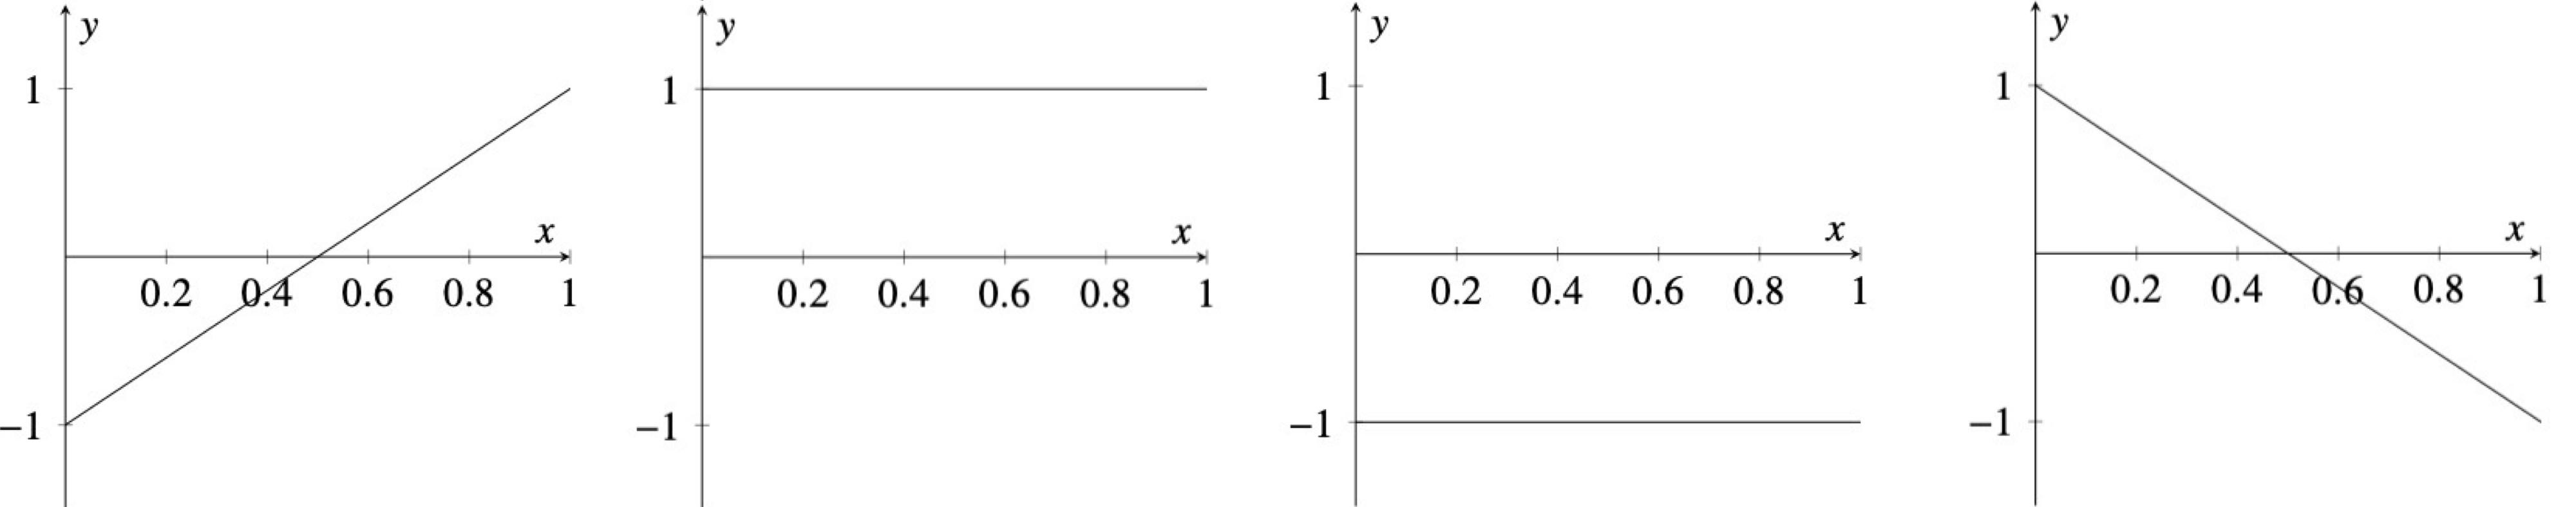
\includegraphics[width=\linewidth]{mainmatter/imgs/states.jpg}
    \caption{visualization of swings, from state1 to state4}
    \label{fig:states}
\end{figure}

Here we display the momentum swings drived from AHP of first three matches.

\begin{figure}[H]
    \centering
    \begin{subfigure}[b]{0.34\textwidth}
        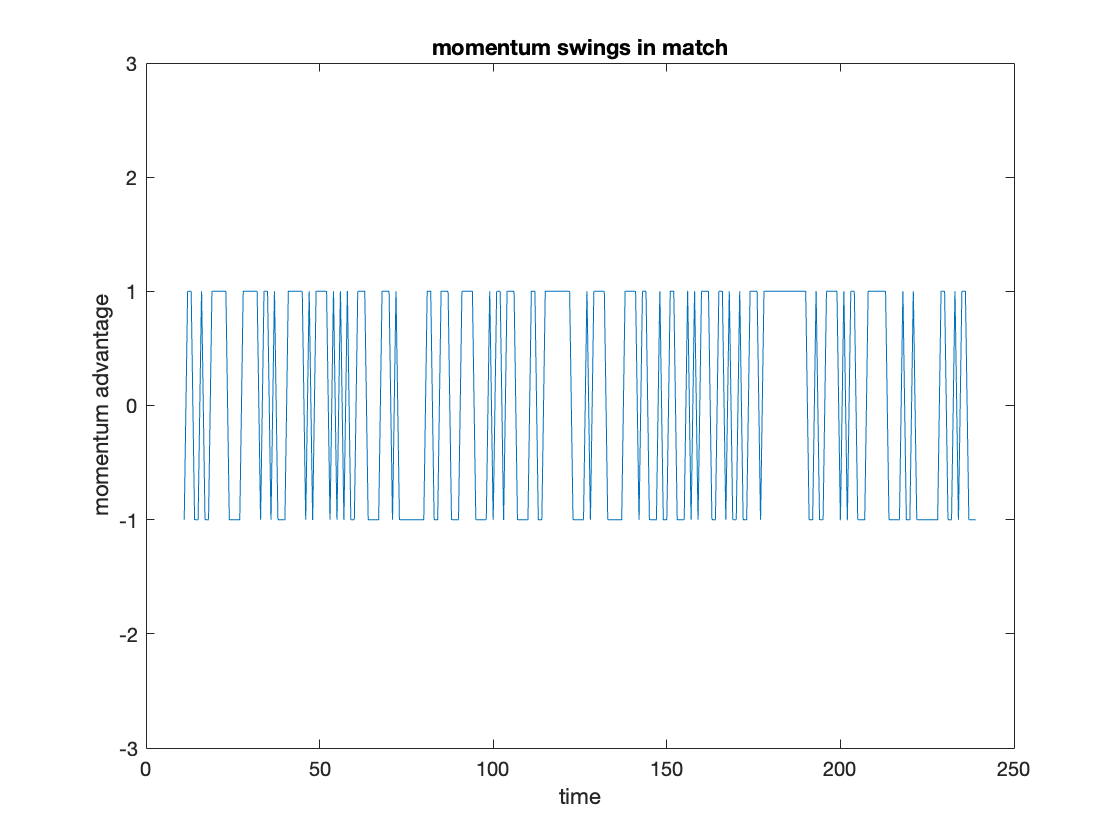
\includegraphics[width=\linewidth]{mainmatter/imgs/swing_match1.png}
        \caption{swings in match 1}
    \end{subfigure}\hspace{-0.02\textwidth}
    \begin{subfigure}[b]{0.34\textwidth}
        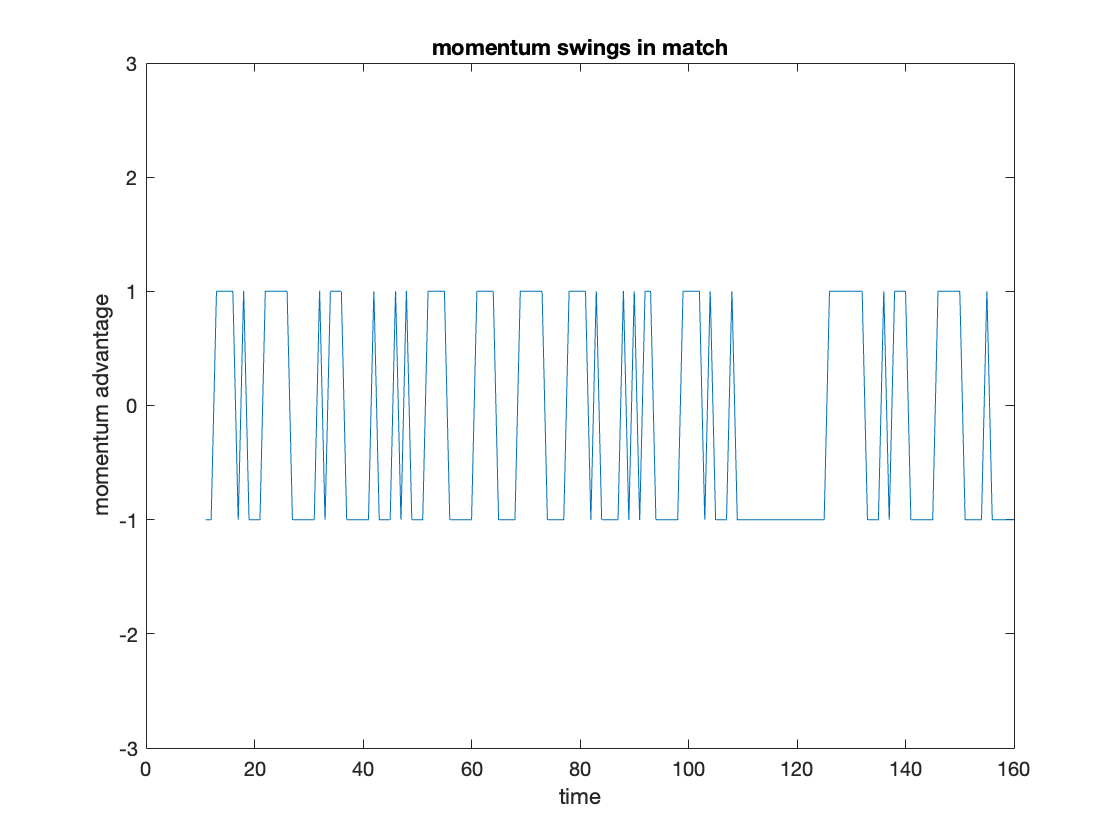
\includegraphics[width=\linewidth]{mainmatter/imgs/swing_match2.png}
        \caption{swings in match 2}
    \end{subfigure}\hspace{-0.02\textwidth}
    \begin{subfigure}[b]{0.34\textwidth}
        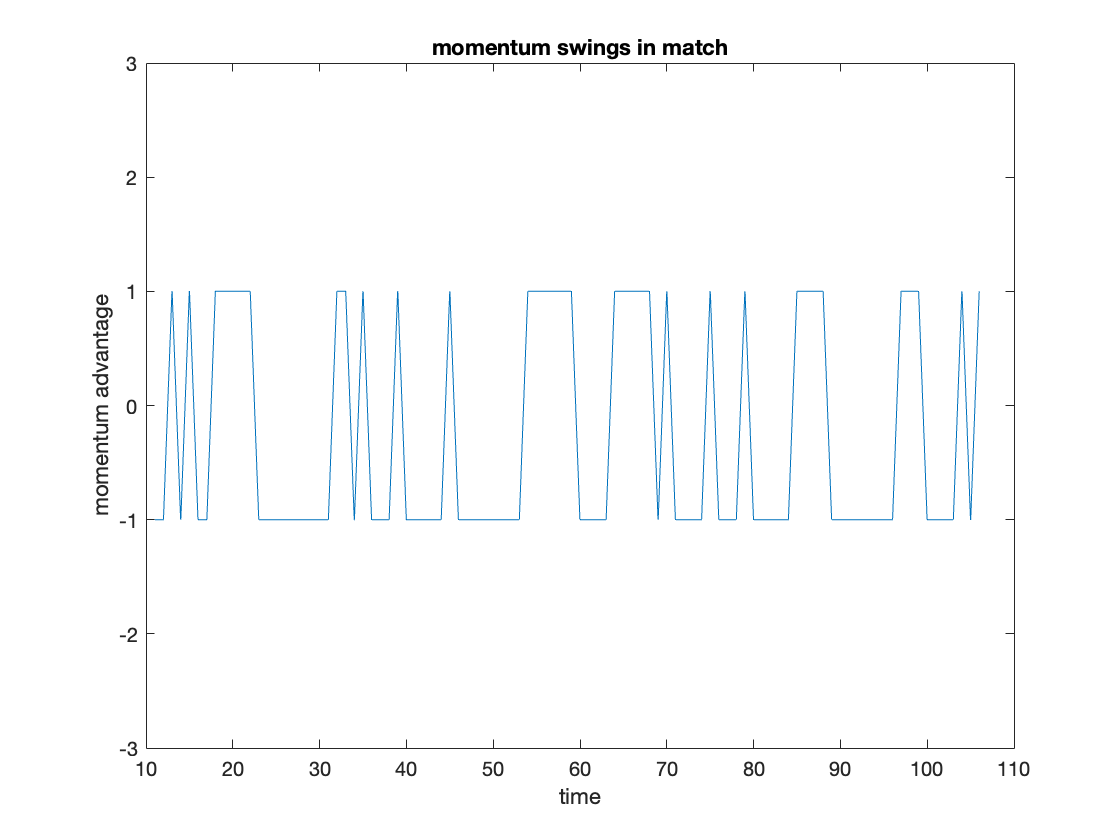
\includegraphics[width=\linewidth]{mainmatter/imgs/swing_match3.png}
        \caption{swings in match 3}
    \end{subfigure}
    \caption{swings in first three matches}
    \label{fig:swings in matches}
\end{figure}


\subsubsection{Data and Label used to train GRU}~{}

To verify all potential factors, meanwhile avoiding over-fitting due to the large number of features,
the data's feature we select is \dots

What's more, we want to find out can swings merely be predicted by the technical data,
so that we can give advice to players on skills,
therefore we delete \verb|scored_last_point, score_diff, game_victor, set_victor| before we train a second model.

The label we use is the state of the swing derived from model of AHP.

we use different sets of data to train and derive different models.

\begin{itemize}
    \item First, we will train the model with data from all matches available.
    \item Then, we will train a new model with data from a single player.
    \item Finally, we will train the model with part of available match statistics
\end{itemize}

From the first model, we can find the important factors that affect all players' momentum swings.
From the second model, we can find the important factors that affect 
especially well on that player's momentum swings.
From the third model, we can examine
the generalization ability to accurately predict the swings in irrelevant players and matches.

\subsubsection{Utilizing the Gated Recurrent Unit (GRU) Network}~{}

Gated Recurrent Units (GRUs) are a type of recurrent neural network (RNN) 
architecture that has gained popularity for sequential data processing. 
And it is appropriate for our many(10)-to-many(5) prediction model.

We will focus on a single unit of recurrent neural network to interpret the hidden mathematical principles:
\begin{figure}[H]
    \centering
    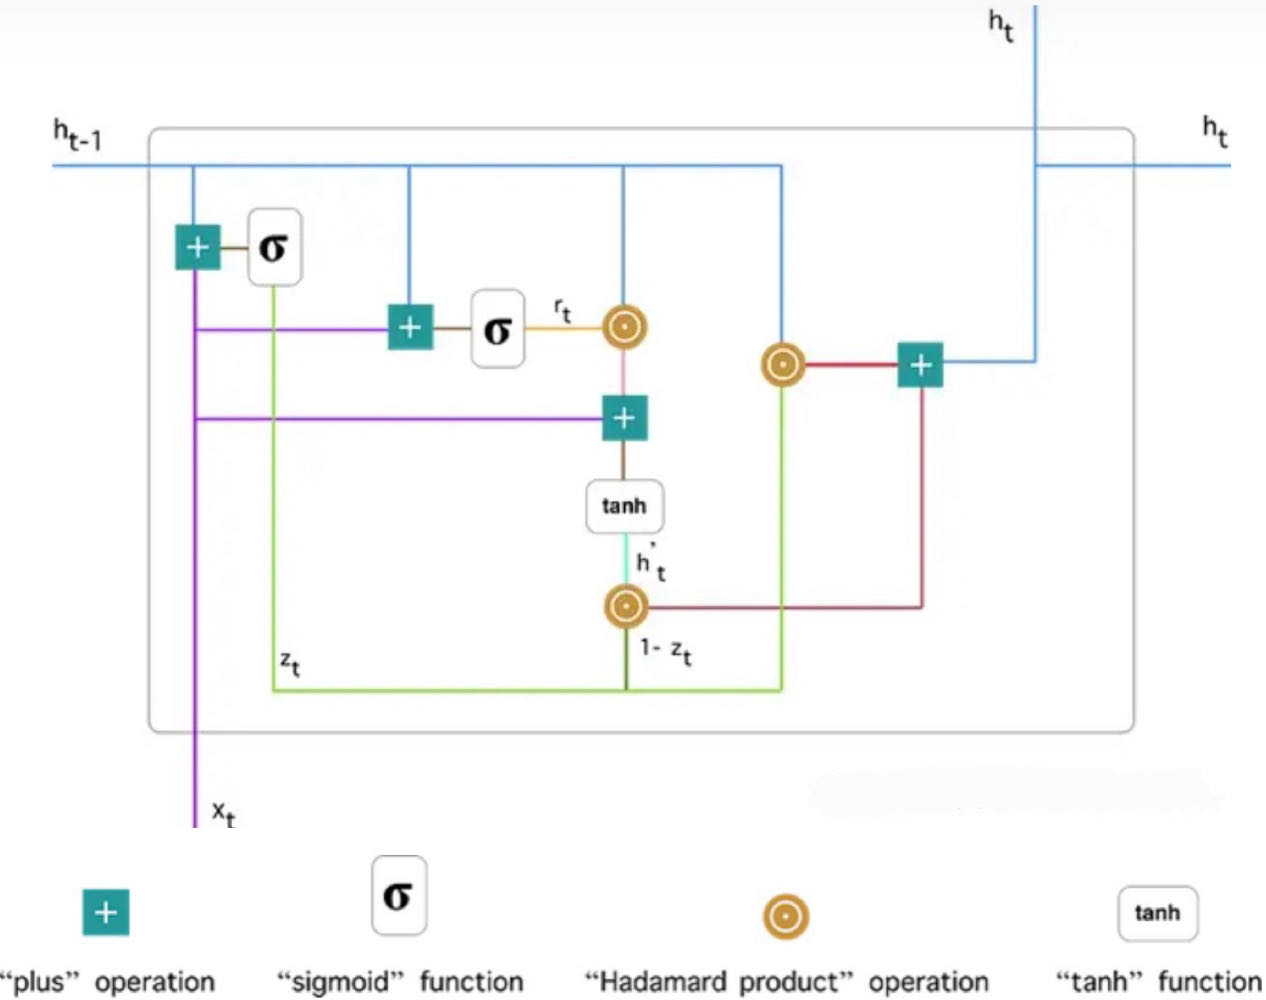
\includegraphics[scale=0.15]{mainmatter/imgs/6.jpg}
    \caption{Structure of GRU}
\end{figure}

\begin{enumerate}
    \item 
    The update gate at time step $t$ is computed using the following formula:  
    $$  z_t = \sigma(W_z \cdot x_t + U_z \cdot h_{t-1})  $$  
    Here, when $x_t$ is input to the network unit, 
    it is multiplied by its own weight $W_z$. 
    Similarly, $h_{t-1}$, which holds the information from the previous $t-1$ units, 
    is multiplied by its own weight $U_z$. These two results are then summed together 
    and passed through a sigmoid activation function to compress the result between 0 and 1. 
  
    \item 
    The essence of the reset gate is for the model to decide how much past information to forget. To compute it, we use:  
    $$  r_t = \sigma(W_r \cdot x_t + U_r \cdot h_{t-1})  $$  

    \item 
    The computation of the new memory content using the reset gate is as follows:  
    $$ h_t'= tanh(Wx_t+r_t\odot Uh_{t-1})$$

    \item 
    The computation for the new memory content $h_t$ using the update gate is as follows:  
    $$ h_t=z_t\odot h_{t-1}+(1-z_t)\odot h_t'$$ 
\end{enumerate}

So, we can predict the momentum swings from the technical data of the past 10 points.

\subsection{Visualization and Analysis}~{}

Out of simplicity, the model shown in this section is trained merely on technical data.

First, we display the model trained on all matches available to 
predict the swings of the play on test data.
To avoid dazzling figure, we minus the swing from AHP with prediction, showing the difference.

Here's the difference of first three matches on training data.

\begin{figure}[H]
    \centering
    \begin{subfigure}[b]{0.34\textwidth}
        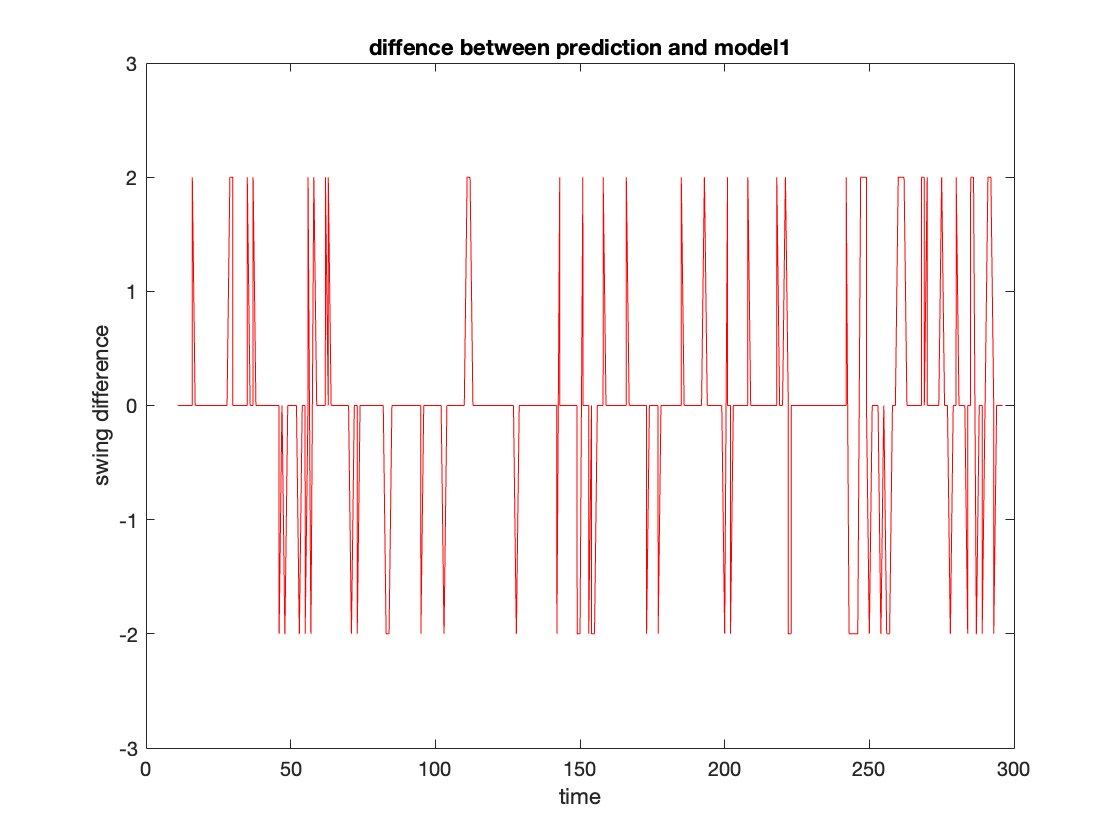
\includegraphics[width=\linewidth]{mainmatter/imgs/swing_diff_match1_overfit.png}
        \caption{difference in match 1}
    \end{subfigure}\hspace{-0.02\textwidth}
    \begin{subfigure}[b]{0.34\textwidth}
        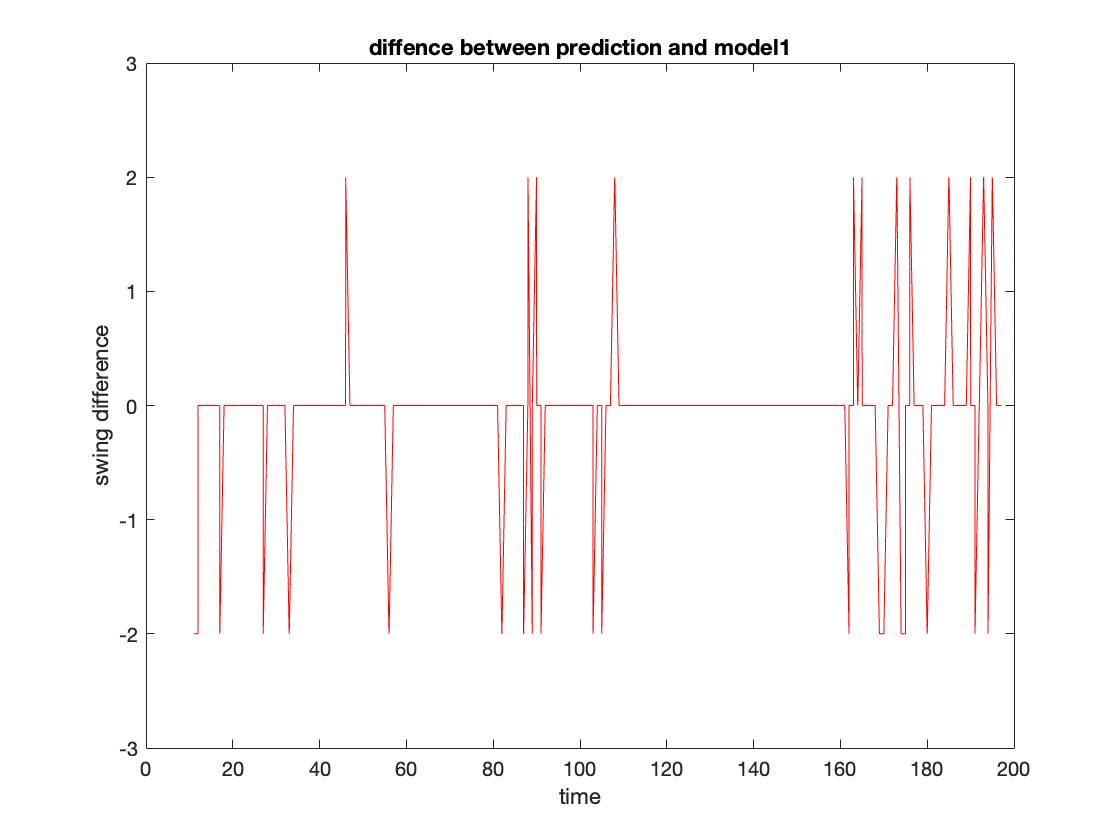
\includegraphics[width=\linewidth]{mainmatter/imgs/swing_diff_match2_overfit.png}
        \caption{difference in match 2}
    \end{subfigure}\hspace{-0.02\textwidth}
    \begin{subfigure}[b]{0.34\textwidth}
        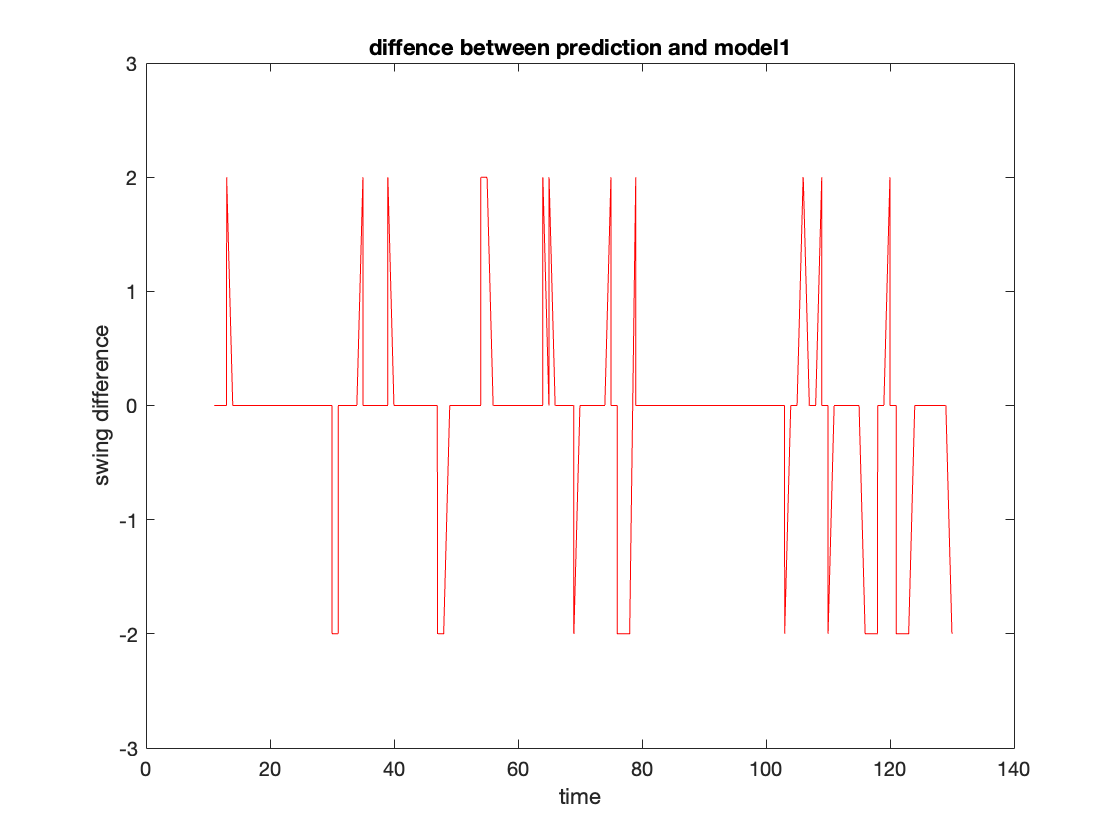
\includegraphics[width=\linewidth]{mainmatter/imgs/swing_diff_match3_overfit.png}
        \caption{difference in match 3}
    \end{subfigure}
    \caption{difference between prediction and AHP model}
    \label{fig:diff swing}
\end{figure}

Here's the difference of first three matches on test data.

calculate the match percentage of each match between the prediction model and the result from AHP.

\subsection{Weight of Factors}

Permutation Feature Importance theory is used to measure the importance of a feature by calculating 
the increase in the model's prediction error after permuting the feature.

Using the above argorithm, we sort FI and normalize them, then we plot the figure:

\begin{figure}[H]
    \centering
    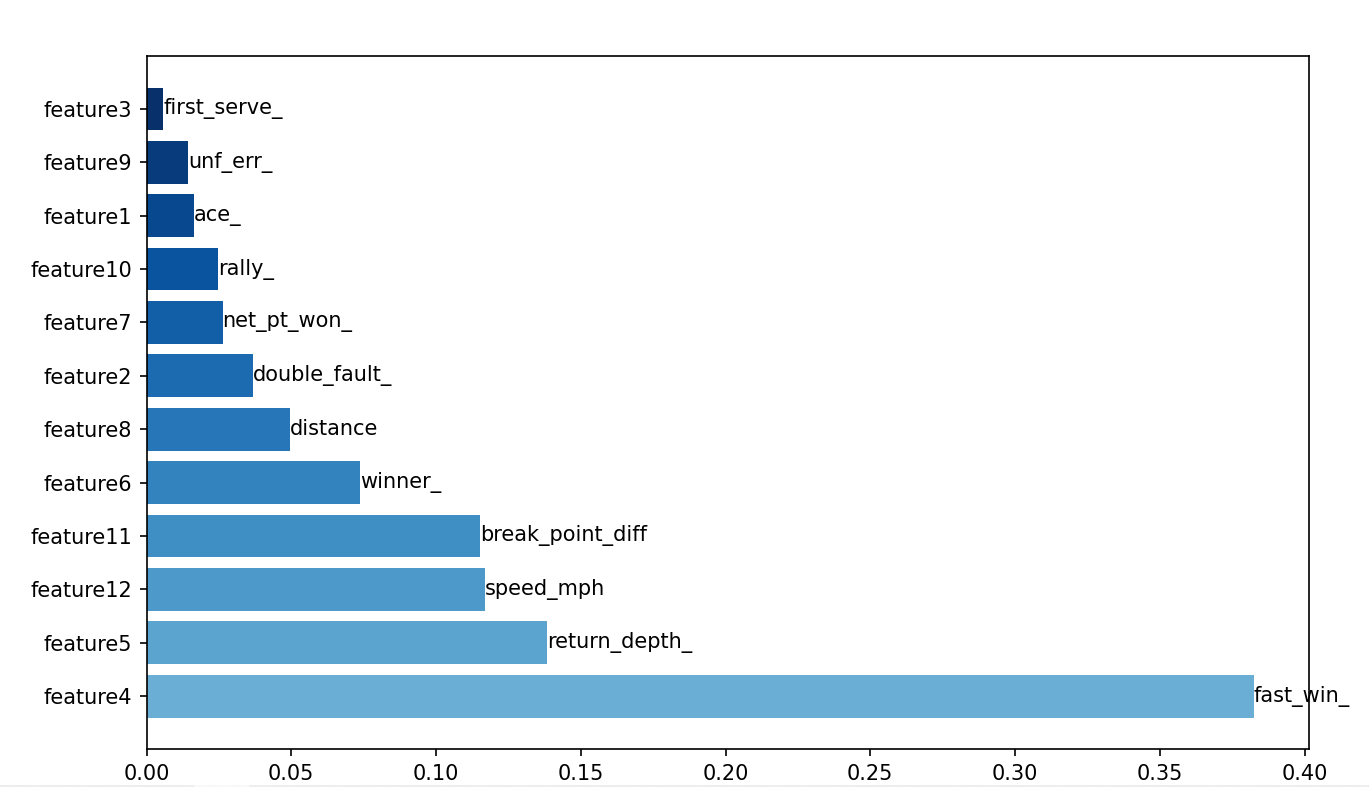
\includegraphics[scale=0.6]{mainmatter/imgs/8.png}
    \caption{feature importance}
\end{figure}

We can see that the most important feature is fast win(rally count < 3 and wins the point),
and the second most important feature is unforced error. Compared to problem 1(main skill features are
running distance, unforced error and fast win),they coincide. The running distance become insignificant, 
we think it is because this factor is also related to fast win.

\subsubsection{Permutation Feature Importance theory}~{}

We measure the importance of a feature by calculating the increase in the model’s prediction error 
after permuting the feature. A feature is “important” if shuffling its values increases the model error, 
because in this case the model relied on the feature for the prediction. A feature is “unimportant” if 
shuffling its values leaves the model error unchanged, because in this case the model ignored the feature 
for the prediction. 

\begin{algorithm}  
    \caption{Permutation Feature Importance}  
    \textbf{Input:} Trained model $\hat{f}$, feature matrix $X$, target vector $y$, error measure $L(y, \hat{f})$.  
      
    Estimate the original model error $e_{orig} = L(y, \hat{f}(X))$ (e.g. mean squared error)  
      
    \textbf{For} each feature $j \in \{1, ..., p\}$ \textbf{do:}  
      
    \quad\quad $\circ$ Generate feature matrix $X_{perm}$ by permuting feature $j$ in the data $X$. This breaks the association between feature $j$ and true outcome $y$.  
      
    \quad\quad $\circ$ Estimate error $e_{perm} = L(Y, \hat{f}(X_{perm}))$ based on the predictions of the permuted data.  
      
    \quad\quad $\circ$ Calculate permutation feature importance as quotient $FI_j = e_{perm} / e_{orig}$ or difference $FI_j = e_{perm} - e_{orig}$  
      
    Sort features by descending FI.
\end{algorithm}

If using match data of multiple different players, the factor with bigger weight is effective to 
all players.

\subsection{Advice against Opponent Based on Weight of Factors}~{}

If using match data of a single player, the factor with bigger weight is extremely effective to 
this player.

Now we choose three players:rublev(three matches), sinner(four matches), alcaraz(five matches), and 
we use the feature analysis method in problem 3 to find their features, the result is as follows:
\begin{figure}[H]
    \centering
    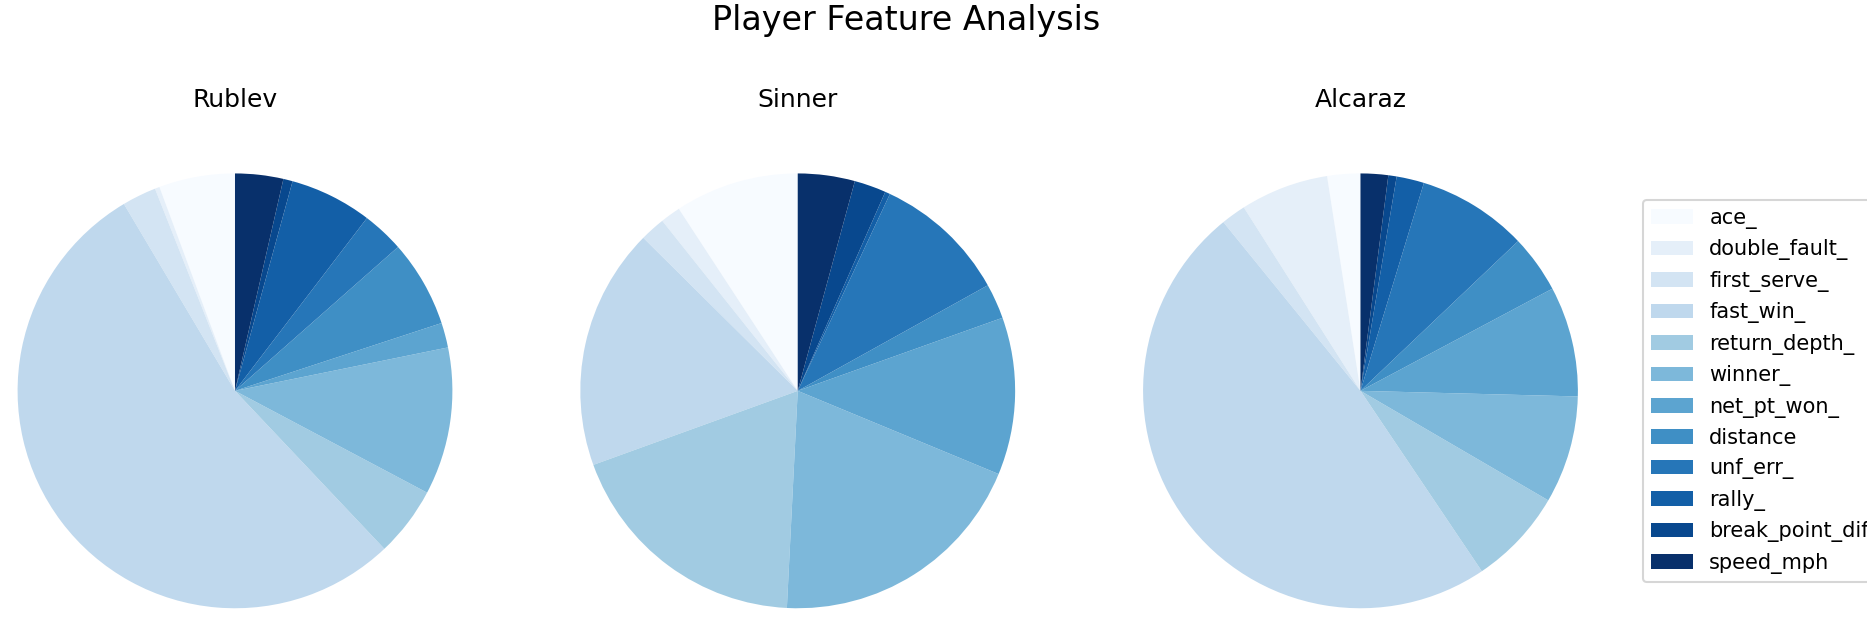
\includegraphics[scale=0.4]{mainmatter/imgs/9.png}
    \caption{features of three players}
\end{figure}
\begin{enumerate}
    \item In comparison to general features, both Rublev and Alcaraz phave significant feature fast win. 
    Therefore, when competing against other players, we recommend them to emphasize the rhythm of seizing 
    the early shots. For example, they can focus more on the quality of their serves, 
    progressively achieving a fast win to enhance their momentum. 
    \item Additionally, Rublev is hardly affected by negative factors such as double fault and 
    unforced error. Hence, in matches, there is no need for him to worry about occasional mistakes; 
    instead, he can play boldly.
    \item For Sinner, his technical characteristics are markedly different. 
    Important features for him are winners and return depth. Consequently, 
    we advise Sinner to fully exploit his strong scoring abilities of winner points
    and utilize his control over return depth to steer the course of the match and establish an advantage.

\end{enumerate}

Now we have finished Problem 3.

\subsection{Prediction Error compared with AHP model outcome}

Overlap rate of the prediction model and the result from AHP is?

\paragraph{Factors we may fail to consider}

First of all, the AHP model is not considering all possible factors to momentum.
For example, the.
So the overlap rate's effectiveness is limited.

Then, from the conclusion of problem 2, momentum only has one order of autocorrelation.
So when we try to predict the far future momentum, there's no reason to be accurate.

\section{Robustness Analysis}

\subsection{Generalization ability}

Now, we have finished Problem 4.

\subsection{Parameters Sensitivity Analysis}

\section{Strength and Weaknesses}

\subsection{Strengths}

\begin{enumerate}
    \item {\bf Visualization in conclusion}: Visualization is used to interpret the result, making it intuitive and concise.
    \item {\bf Proper models chosen}: Two models in problem 1 and problem 3 have similar results of the influencing factors, which makes it more reliable.
    \item {\bf Stable performance}: Our model has stable prediction in different men's matches.
    \item {\bf Classification of different situations}: We evaluate momentum in two different situations, serve and opponent serve.
\end{enumerate}


\subsection{Weaknesses}

\begin{enumerate}
    \item {\bf A little subjective}: In problem 1, AHP is a subjective method to some extent, so although we get desired result similar to problem 3,
    some new completely objective method needs to be carried out.
    \item {\bf Limited ability in predicting other kinds of matches}: The technical indexes are different in other matches, so if we want to predict them, 
    we need to do some modification on our model.
\end{enumerate}

%back matter%%%%%%%%%%%%%%%%%%%%%%%%%
\addcontentsline{toc}{section}{Refences}
\bibliography{backmatter/papers}

\appendix
\section{Advice for Coaches: Understanding and Utilizing Momentum in Tennis Matches}

\paragraph{Introduction}~{}

Momentum in tennis is an intangible yet powerful force that can influence the outcome of a match. Other than the player's skill and ability, having the momentum is often a key to success. It's coaches' duty to prepare players in all aspects to understand and harness momentum, and to respond effectively to events that could impact the flow of play. By understanding momentum and ways to have it at one's side can help coaches identify how and where a match is won and lost.

\paragraph{What exactly is momentum?}~{}

Momentum refers to the perceived shift in advantage or energy favoring one player or another. In other words, momentum reflects which player is going to act strong in the near future.

\paragraph{What are the factors influencing momentum?}~{}

There are many aspects influencing momentum, including the player's current performance statiscally and the current score situation, and each of those two aspects consists of many specific factors. By analyzing the weight of all factors, we found that the current score situation plays a way more important role than the player's skill statistics in affecting momentum. Specificly, the recent score difference most significantly affects the momentum. For example, if the recent score difference is small, the game is a close-game and the momentum is likely to shift.

\paragraph{Why are momentum so easily affected by score?}~{}

This is because the player's mantality plays a very important role on the court. Unlike basketball games, in which coaches can call timeout when they feel they're losing momentum, tennis coaches can't easily do anything in a match to directly interfere with the match. Due to this reason, the player's mindset is prone to shift according to the current score situation, resulting in his performance going through ups and downs in a match, thus affecting momentum.



**Preparation Strategies**

1. **Mental Conditioning**:
   - Implement mental training exercises that simulate pressure situations.
   - Teach players to maintain a positive attitude and focus on the present moment, not past mistakes or future what-ifs.

2. **Routine Development**:
   - Encourage players to establish pre-serve and point routines to maintain a sense of control and normalcy, regardless of the match situation.

3. **Emotional Regulation**:
   - Equip players with strategies to manage emotions. Deep breathing, positive self-talk, and visualization techniques can help regain composure during critical moments.

4. **Scenario Training**:
   - During practice sessions, create scenarios where a player is ahead or behind, to simulate momentum shifts and practice appropriate responses.

**In-Match Strategies**

1. **Recognizing and Exploiting Momentum**:
   - Teach players to capitalize on momentum by increasing their level of assertiveness during play, making high-percentage shots, and keeping opponents under pressure.

2. **Interrupting Opponent's Momentum**:
   - Advise players on tactics to disrupt the opponent's rhythm, such as changing the pace of play, taking legitimate breaks (e.g., to retie shoelaces), or using varied shot selection.

3. **Regaining Lost Momentum**:
   - Instruct players on strategies to regain momentum, such as focusing on one point at a time, sticking to their game plan, and increasing movement to boost energy levels.

**Post-Match Analysis**

1. **Reflect on Momentum Shifts**:
   - After matches, review key moments where momentum shifted. Discuss what led to these shifts and how they were managed.

2. **Continuous Learning**:
   - Use video analysis to study players' responses to momentum changes and identify areas for improvement.

**Conclusion**

Momentum is a subtle yet critical aspect of the game that can dictate the ebb and flow of a tennis match. By preparing our players mentally and strategically to handle momentum swings, we can significantly improve their ability to perform under pressure and influence the match's outcome in their favor. Let's integrate these practices into our training sessions and match day routines to build players' resilience and adaptability.

**Action Item**: Please incorporate the mentioned strategies into your training plans and discuss any individual player's needs with me at your earliest convenience.

Best Regards,

[Your Name]
[Your Position]

\section{report on Use of AI}

\cite{Alice13}

1.

OpenAI ChatGPT (Feb 2,2024 version,ChatGPT3.5)

Query1:  \emph{
    “swings in play and runs of success by one player are random” 
can this sentence to be interpreted as  swings in play and runs of success by one player are independent?
}

Output: \emph{Yes, the sentence "swings in play and runs of success by one player are random" 
can be interpreted as suggesting that swings in play and runs of success by one player are 
independent of each other. In statistical terms, independence means that the occurrence or 
outcome of one event does not influence the occurrence or outcome of another.}

\emph{
In the context of tennis, this would imply that the fluctuations in the dynamics of the match 
(swings in play) and a player's success streaks (runs of success) are not connected or dependent 
on each other. Each event is considered random and not influenced by the occurrence of the other.
}

\end{document}